% Rascunho PT-BR gerado a partir do passe de trabalho espanhol congelado; a fonte permanece em source_es.
% SGA 3, Tomo II — Exposé IX. Ordem canônica da tradução brasileira.
% SGA 3, Exposé IX, tradução brasileira.
% Escopo: título e §1 integral.
% Autoridade: Polo--Gille Exp9-8nov09.pdf, pp. locais 1--3,
% leitor completo pp. 647--649, pp. impressas 37--40.
% O TeX inglês serve unicamente para o alinhamento estrutural; o PDF francês
% controla o texto, as fórmulas, a numeração e as notas.

\setcounter{footnote}{-1}
\SGARefTarget{sga3:ix:chapter:ix}\chapter*{Exposé IX\\
Grupos de tipo multiplicativo:\\
Homomorfismos em um esquema em grupos}
\addcontentsline{toc}{chapter}{Exposé IX. Grupos de tipo multiplicativo:
homomorfismos em um esquema em grupos}
\markboth{EXPOSÉ IX. GRUPOS DE TIPO MULTIPLICATIVO I (HOMOMORFISMOS)}
  {EXPOSÉ IX. GRUPOS DE TIPO MULTIPLICATIVO I (HOMOMORFISMOS)}

\begin{center}
  \textit{por A. Grothendieck}\footnote{Nota do editor: versão 1.0 de
  8 de novembro de 2009. Fizeram-se acréscimos na demonstração de
  \SGARefLink{sga3:ix:theorem:3:6:bis}{3.6 bis}, em
  \SGARefLink{sga3:ix:lemma:4:4}{4.4}--\SGARefLink{sga3:ix:theorem:4:7}{7},
  \SGARefLink{sga3:ix:lemma:5:0}{5.0}--\SGARefLink{sga3:ix:theorem:5:6}{6},
  \SGARefLink{sga3:ix:lemma:6:1}{6.1},
  \SGARefLink{sga3:ix:theorem:7:1}{7.1} e
  \SGARefLink{sga3:ix:proposition:8:2}{8.2}. Restam por revisar
  \SGARefLink{sga3:ix:proposition:8:1}{8.1} e
  \SGARefLink{sga3:ix:lemma:4:5}{4.5}.}
\end{center}

\SGARefTarget{sga3:ix:section:1}\section*{1. Definições}
\addcontentsline{toc}{section}{1. Definições}

% Página-fonte: Exp9 p. local 1; leitor completo p. 647; p. impressa 37.
\medskip
\noindent\SGARefTarget{sga3:ix:definition:1:1}\textbf{Definição 1.1.} ---
\textit{Seja \(S\) um pré-esquema e seja \(G\) um pré-esquema em grupos sobre
\(S\). Diz-se que o grupo \(G\) é \emph{de tipo multiplicativo} se for
localmente diagonalizável para a topologia fielmente plana e
quase compacta (cf.\ \SGARefLink{sga3:iv:subsection:6:3}{IV 6.3}); isto é,
se, para todo \(s\in S\), existem uma vizinhança aberta \(U\) de \(s\) e um
morfismo fielmente plano e quase compacto \(S'\to U\) tais que}
\[
  G'=G\times_S S'
\]
\textit{seja um \(S'\)-grupo diagonalizável
(\SGARefLink{sga3:i:subsection:4-4}{I 4.4} e
\SGARefLink{sga3:viii:definition:1:1}{VIII 1.1}).}

\textit{Diz-se que o grupo \(G\) é \emph{de tipo multiplicativo
quase-isotrivial} se for localmente diagonalizável até mesmo para a topologia
étale (\SGARefLink{sga3:iv:subsection:6:3}{IV 6.3}); isto é, se, na
definição precedente, se puder tomar \(S'\to U\) étale e sobrejetivo. De
maneira equivalente ---como se vê tomando a união disjunta dos esquemas
\(S'\) associados aos diversos \(s\in S\)---, existe um morfismo étale
sobrejetivo \(S'\to S\) tal que \(G'=G\times_S S'\) seja um \(S'\)-grupo
localmente diagonalizável.}

\textit{Se, além disso, for possível escolher \(S'\to S\) finito, étale e
sobrejetivo, diz-se que \(G\) é \emph{de tipo multiplicativo
isotrivial}.}

\textit{Por fim, diz-se que \(G\) é um grupo \emph{de tipo
multiplicativo localmente trivial} (respectivamente, \emph{de tipo
multiplicativo localmente isotrivial}) se todo \(s\in S\) possuir uma vizinhança
aberta \(U\) tal que \(G\times_S U\) seja um \(U\)-grupo diagonalizável
(respectivamente, seja de tipo multiplicativo isotrivial; dito de outro
modo, existe um morfismo finito étale sobrejetivo \(S'\to U\) tal que
\(G\times_S S'\) seja um \(S'\)-grupo diagonalizável).}

\medskip
\noindent\SGARefTarget{sga3:ix:comments:1:2}\textbf{Comentários 1.2.} ---
As cinco noções precedentes são todas obtidas, por localização, a partir
da noção de grupo diagonalizável, com respeito a cinco «topologias»
distintas associadas a \((\mathbf{Sch})\).

Subentende-se, em geral, que, quando a palavra «localmente» não é
precisada pelo nome da topologia considerada, trata-se da topologia de
Zariski, em conformidade com a terminologia estabelecida. Na terminologia
aqui introduzida, «de tipo multiplicativo localmente trivial» equivale a
«localmente diagonalizável» em
\SGARefLink{sga3:viii:definition:1:1}{VIII 1.1}; do mesmo modo, «trivial»
traduz-se por «diagonalizável». As cinco noções introduzidas se dispõem no
diagrama de implicações seguinte, que resulta das relações correspondentes
entre as topologias consideradas:

% Página-fonte: Exp9 p. local 2; leitor completo p. 648; pp. impressas 38--39.
\SGARefTarget{sga3:ix:diagram:1:2}
\begin{center}
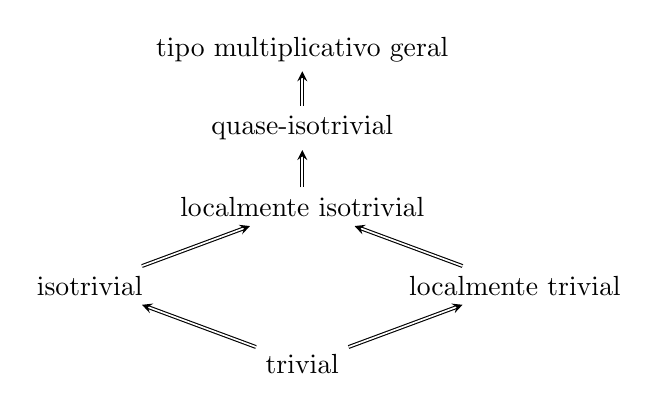
\begin{tikzpicture}[>=stealth]
  \node (general) at (0,4.0) {tipo multiplicativo geral};
  \node (quasi) at (0,3.0) {quase-isotrivial};
  \node (lociso) at (0,2.0) {localmente isotrivial};
  \node (iso) at (-2.7,1.0) {isotrivial};
  \node (loctriv) at (2.7,1.0) {localmente trivial};
  \node (triv) at (0,0) {trivial};
  \draw[double,->] (quasi) -- (general);
  \draw[double,->] (lociso) -- (quasi);
  \draw[double,->] (iso) -- (lociso);
  \draw[double,->] (loctriv) -- (lociso);
  \draw[double,->] (triv) -- (iso);
  \draw[double,->] (triv) -- (loctriv);
\end{tikzpicture}
\end{center}

Para as aplicações, assinalemos desde já que todo grupo de tipo
multiplicativo que encontrarmos será quase-isotrivial. Com efeito, veremos na
exposição seguinte (\SGARefLink{sga3:x:corollary:4-5}{X 4.5}) que,
quando \(G\) é de tipo finito sobre \(S\), ele é automaticamente
quase-isotrivial; daremos, contudo, exemplos nos quais não é localmente
isotrivial. Veremos igualmente que \(G\) pode ser localmente trivial sem ser
isotrivial e, portanto, \emph{a fortiori}, sem ser trivial. Daí se
deduz facilmente que as inclusões do
\SGARefLink{sga3:ix:diagram:1:2}{diagrama precedente} são estritas.

Por outro lado, veremos também ali
(\SGARefLink{sga3:x:theorem:5-16}{X 5.16}) que, se \(S\) é localmente
noetheriano e normal ---ou, mais geralmente, geometricamente
unirramoso---, todo grupo de tipo multiplicativo e de tipo finito sobre
\(S\) é necessariamente isotrivial; além disso, é trivial assim que for
localmente trivial (ou mesmo meramente trivial sobre um aberto denso).
Isso explica por que a maioria dos grupos de tipo multiplicativo que
aparecem na prática será, sem dúvida, isotrivial, tanto mais que
veremos adiante que os toros maximais dos esquemas em grupos
semissimples são automaticamente isotriviais.

\medskip
\noindent\SGARefTarget{sga3:ix:definition:1:3}\textbf{Definição 1.3.} ---
\textit{Sejam \(S\) e \(G\) como em
\SGARefLink{sga3:ix:definition:1:1}{1.1}. Chama-se \emph{toro} o grupo
\(G\) se, para a topologia fielmente plana e quase compacta, ele for localmente
isomorfo a um grupo da forma \(\mathbf G_m^r\), onde \(r\) é um
inteiro tal que \(r\geq0\).}

Com as notações de \SGARefLink{sga3:ix:definition:1:1}{1.1}, isso
significa que se pode escolher \(S'\) de modo que \(G'\) seja isomorfo a um
grupo da forma \((\mathbf G_{m,S'})^r\). O inteiro \(r\) depende de
\(s\in S\): é a dimensão da fibra
\[
  G_s=G\otimes_S\kappa(s).
\]
É uma função localmente constante de \(s\), como se vê imediatamente.
Essa observação deve ser generalizada da maneira seguinte.

% Página-fonte: Exp9 p. local 3; leitor completo p. 649; pp. impressas 39--40.
\medskip
\noindent\SGARefTarget{sga3:ix:definition:1:4}\textbf{Definição 1.4.} ---
\textit{Seja \(G\) um esquema em grupos diagonalizável sobre um corpo
\(k\). Assim, \(G\) é isomorfo a um grupo \(D_k(M)\), onde \(M\) é um
grupo comutativo ordinário determinado, a menos de isomorfismo, por essa
condição; mais precisamente,}
\[
  M\simeq\operatorname{Hom}_{k\text{-}\mathrm{gr}}
    (G,\mathbf G_{m,k})
\]
\textit{(\SGARefLink{sga3:viii:corollary:1:3}{VIII 1.3}). A classe de
isomorfismo de \(M\) chama-se o \emph{tipo} do grupo diagonalizável
\(G\); ela é manifestamente invariante por extensão do corpo de base.}

\textit{Seja agora \(G\) um esquema em grupos de tipo multiplicativo sobre
um pré-esquema qualquer \(S\). Para todo \(s\in S\), existe uma extensão
\(k\) de \(\kappa(s)\) tal que
\(G\times_S\operatorname{Spec}(k)\) seja um \(k\)-grupo
diagonalizável.\footnote{Nota do editor: com efeito, por hipótese existem
uma vizinhança aberta \(U\) de \(s\) e um morfismo fielmente plano e
quase compacto \(S'\to U\) tais que \(G_{S'}\) é diagonalizável. Para todo
\(s'\in S'\) sobre \(s\), o corpo \(\kappa(s')\) é uma extensão de
\(\kappa(s)\), e
\(G_{s'}=G\times_S\operatorname{Spec}(\kappa(s'))\) é diagonalizável.}
Seu tipo independe da extensão escolhida, pela observação
precedente, e chama-se o \emph{tipo de \(G\) em \(s\)}, ou o \emph{tipo
de \(G_s\)}. Em particular, se o próprio \(G\) é diagonalizável e, portanto,
isomorfo a um grupo da forma \(D_S(M)\), então, para todo \(s\in S\),
o tipo de \(G\) em \(s\) é a classe de isomorfismo de \(M\).}

\textit{Mais geralmente, se \(G\) é um grupo de tipo multiplicativo
sobre \(S\) e \(M\) é um grupo comutativo ordinário, diz-se que \(G\)
é \emph{de tipo \(M\)} se for de tipo \(M\) em todo ponto \(s\in S\); de
maneira equivalente, se \(G\) for localmente isomorfo a \(D_S(M)\) para a
topologia fielmente plana e quase compacta.}

\medskip
\noindent\SGARefTarget{sga3:ix:remark:1:4:1}\textbf{Observação 1.4.1.}
\footnote{Nota do editor: acrescentou-se o número
\SGARefLink{sga3:ix:remark:1:4:1}{1.4.1} às observações seguintes,
para que pudessem ser citadas posteriormente.}
\SGARefTarget{sga3:ix:remark:1:4:1:item:a}\textit{a) Para um grupo \(G\)
de tipo multiplicativo sobre \(S\), a função}
\[
  s\longmapsto \text{el tipo de }G_s
\]
\textit{é localmente constante sobre \(S\). Com efeito, com as notações
de \SGARefLink{sga3:ix:definition:1:1}{1.1}, se \(G'\) é de tipo \(M\),
então \(G\) é de tipo \(M\) sobre a vizinhança \(U\) de \(s\). Por
conseguinte, \(S\) possui uma decomposição canônica como união disjunta de
pré-esquemas \(S_i\) tais que, para todo \(i\), \(G_{S_i}\) é de tipo
\(M_i\), onde os grupos comutativos \(M_i\) não são isomorfos dois a dois.}

\SGARefTarget{sga3:ix:remark:1:4:1:item:b}\textit{b) Em particular, se
\(S\) é conexo, o tipo das fibras de \(G\) é constante; isto é,
existe um grupo comutativo \(M\) tal que \(G\) é de tipo \(M\). Por
fim, se \(G\) é um toro, o tipo de \(G\) em \(s\) é determinado
pelo inteiro \(\dim G_s\): com efeito, \(G_s\) é de tipo \(\mathbb Z^n\),
onde \(n=\dim G_s\).}

\medskip
\noindent\SGARefTarget{sga3:ix:remark:1:5}\textbf{Observação 1.5.} ---
\SGARefTarget{sga3:ix:remark:1:5:item:a}\textit{a) Das Definições
\SGARefLink{sga3:ix:definition:1:1}{1.1} e
\SGARefLink{sga3:ix:definition:1:3}{1.3} segue imediatamente que essas
noções são «compatíveis com a extensão da base». Assim, se \(G\) é
um pré-esquema em grupos sobre \(S\) e \(S'\to S\) é um morfismo de mudança
de base, então, sempre que \(G\) for de tipo multiplicativo
(respectivamente, de tipo multiplicativo isotrivial etc.), o mesmo valerá
para \(G'\).}

\SGARefTarget{sga3:ix:remark:1:5:item:b}\textit{b) Se, além disso, \(S'\to S\)
é fielmente plano e quase compacto, o fato de \(G'\) ser de tipo
multiplicativo, respectivamente um toro, implica o mesmo para \(G\). Se
\(S'\to S\) também é étale (respectivamente, finito étale), o fato de
\(G'\) ser quase-isotrivial (respectivamente, isotrivial) implica o
mesmo para \(G\).}

\SGARefTarget{sga3:ix:remark:1:5:item:c}\textit{c) Voltemos, por fim, a
um morfismo de mudança de base qualquer \(f:S'\to S\). Se \(s'\in S'\) e
\(s=f(s')\), o tipo de \(G'\) em \(s'\) é o mesmo que o de \(G\) em
\(s\), pois}
\[
  G'_{s'}=G_s\otimes_{\kappa(s)}\kappa(s').
\]

% SGA 3, Exposé IX, tradução brasileira.
% Escopo: §2 integral.
% Autoridade: Polo--Gille Exp9-8nov09.pdf, pp. locais 4--7,
% leitor completo pp. 650--653, pp. impressas 41--46.

\setcounter{footnote}{2}

\SGARefTarget{sga3:ix:section:2}\section*{2. Extensão de certas
propriedades dos grupos diagonalizáveis aos grupos de tipo
multiplicativo}
\addcontentsline{toc}{section}{2. Extensão de certas propriedades dos
grupos diagonalizáveis aos grupos de tipo multiplicativo}

As extensões em questão são consequências essencialmente triviais
dos resultados da Exposição precedente, levando-se em conta
\SGARefLink{sga3:ix:definition:1:1}{as definições de 1.1} e o caráter
«local» (para a topologia fielmente plana e quase compacta) dos
resultados considerados.

\medskip
\noindent\SGARefTarget{sga3:ix:definition:2:0}\textbf{Definição 2.0.}
\footnote{Nota do editor: acrescentou-se esta definição; ela intervém nas
Proposições~\SGARefLink{sga3:ix:proposition:2:3}{2.3} e
\SGARefLink{sga3:ix:proposition:2:7}{2.7}.}
\textit{Denotamos por \(\mathcal M\) o conjunto dos morfismos
fielmente planos e quase compactos.}

\medskip
\noindent\SGARefTarget{sga3:ix:proposition:2:1}\textbf{Proposição 2.1.}
\textit{Seja \(G\) um grupo de tipo multiplicativo sobre um pré-esquema
\(S\). Então:}
\begin{enumerate}
  \item[(a)]\SGARefTarget{sga3:ix:proposition:2:1:item:a:01}
  \textit{\(G\) é fielmente plano sobre \(S\) e afim sobre \(S\)
  (\emph{a fortiori}, quase compacto sobre \(S\));}

  \item[(b)]\SGARefTarget{sga3:ix:proposition:2:1:item:b:01}
  \textit{\(G\) é de tipo finito sobre \(S\) se, e somente se, é de
  apresentação finita sobre \(S\), se, e somente se, para todo \(s\in S\),
  o tipo de \(G\) em \(s\) é dado por um grupo comutativo de tipo
  finito;}

  \item[(c)]\SGARefTarget{sga3:ix:proposition:2:1:item:c:01}
  \textit{\(G\) é finito sobre \(S\) se, e somente se, para todo
  \(s\in S\), o tipo de \(G\) em \(s\) é dado por um grupo
  comutativo finito, se, e somente se (quando \(S\) é quase compacto), \(G\)
  é de tipo finito sobre \(S\) e é anulado por um inteiro \(n>0\);}

  \item[\((c')\)]\SGARefTarget{sga3:ix:proposition:2:1:item:cprime:01}
  \textit{\(G\) é inteiro sobre \(S\) se, e somente se, para todo
  \(s\in S\), o tipo de \(G\) em \(s\) é dado por um grupo
  comutativo de torção;}

  \item[(d)]\SGARefTarget{sga3:ix:proposition:2:1:item:d:01}
  \textit{\(G\) é o grupo unidade se, e somente se, para todo \(s\in S\),
  o tipo de \(G\) em \(s\) é dado pelo grupo comutativo zero;}

  \item[(e)]\SGARefTarget{sga3:ix:proposition:2:1:item:e:01}
  \textit{\(G\) é liso sobre \(S\) se, e somente se, para todo \(s\in S\),
  o tipo de \(G\) em \(s\) é dado por um grupo comutativo de tipo
  finito cujo subgrupo de torção tem ordem prima com a característica
  de \(\kappa(s)\).}
\end{enumerate}

Essas afirmações deduzem-se de
\SGARefLink{sga3:viii:proposition:2:1}{VIII~2.1}, levando em conta que
as propriedades em questão descendem por morfismos fielmente planos e
quase compactos (cf. SGA~1, VIII, ou EGA~IV\textsubscript{2}, \S2).

Utilizando \SGARefLink{sga3:viii:corollary:3:5}{VIII~3.5}, obtém-se
também:

\medskip
\noindent\SGARefTarget{sga3:ix:proposition:2:2}\textbf{Proposição 2.2.}
\textit{Seja \(G\) um grupo de tipo multiplicativo e de tipo finito sobre
\(S\). Para todo inteiro \(n\ne0\), o núcleo
\({}_nG=\ker(n\cdot\operatorname{id}_G)\) é um grupo de tipo
multiplicativo, finito sobre \(S\).}

\medskip
\noindent\SGARefTarget{sga3:ix:proposition:2:3}\textbf{Proposição 2.3.}
\textit{Seja \(G\) um grupo de tipo multiplicativo sobre o pré-esquema
\(S\), que atua livremente à direita sobre um \(S\)-pré-esquema
\(X\), afim sobre \(S\). Então:}
\begin{enumerate}
  \item[(a)]\SGARefTarget{sga3:ix:proposition:2:3:item:a:01}
  \textit{a relação de equivalência definida por \(G\) em \(X\) é
  \(\mathcal M\)-efetiva
  (\SGARefLink{sga3:iv:subsection:3:4}{IV~3.4}), e \(Y=X/G\) é afim
  sobre \(S\);}

  \item[(b)]\SGARefTarget{sga3:ix:proposition:2:3:item:b:01}
  \textit{se, além disso, \(X\) é de apresentação finita (respectivamente,
  de tipo finito) sobre \(S\), o mesmo vale para \(Y\).}
\end{enumerate}

\SGARefLink{sga3:ix:proposition:2:3:item:a:01}{A primeira afirmação}
deduz-se de \SGARefLink{sga3:viii:theorem:5:1}{VIII~5.1}, que trata do caso
em que \(G\) é diagonalizável, e de
\SGARefLink{sga3:iv:proposition:3:5:2}{IV~3.5.2}, que permite reduzir-se a
esse caso. Com efeito, os morfismos fielmente planos e quase compactos
\(S'\to S\) são morfismos de descida efetiva para a categoria fibrada
dos esquemas afins sobre os esquemas: se \(Y'\) é afim sobre \(S'\)
e está munido de um dado de descida relativo a \(S'\to S\), esse dado
é efetivo, isto é, \(Y'\) provém de um esquema \(Y\) afim sobre
\(S\) (cf. SGA~1, \SGARefLink{sga3:viii:proposition:2:1}{VIII~2.1}).

% Página-fonte: Exp9 p. local 5; leitor completo p. 651; p. impressa 43.
Para \SGARefLink{sga3:ix:proposition:2:3:item:b:01}{a segunda afirmação},
reduz-se igualmente ao caso diagonalizável de
\SGARefLink{sga3:viii:corollary:5:8}{VIII~5.8}, pois as condições de
finitude consideradas descendem por morfismos fielmente planos e
quase compactos (SGA~1, VIII~3.3 e 3.6\footnote{Nota do editor: veja-se
também V, 9.1, ou EGA~IV\textsubscript{2}, 2.7.1.}). Procedendo como em
VIII, Corolários~5.5--5.7, deduz-se de
\SGARefLink{sga3:ix:proposition:2:3}{2.3}:

\medskip
\noindent\SGARefTarget{sga3:ix:corollary:2:4}\textbf{Corolário 2.4.}
\textit{Sob as hipóteses de
\SGARefLink{sga3:ix:proposition:2:3}{2.3}, o morfismo gráfico}
\SGARefTarget{sga3:ix:corollary:2:4:diagram:01}
\[
  X\times_S G\longrightarrow X\times_S X
\]
\textit{é uma imersão fechada. Para toda seção \(\sigma\) de \(X\)
sobre \(S\), o morfismo correspondente}
\[
  G\longrightarrow X,\qquad g\longmapsto\sigma\cdot g,
\]
\textit{é uma imersão fechada.}

Em particular:

\medskip
\noindent\SGARefTarget{sga3:ix:corollary:2:5}\textbf{Corolário 2.5.}
\textit{Seja \(u:G\to H\) um monomorfismo de \(S\)-pré-esquemas em grupos,
com \(G\) de tipo multiplicativo e \(H\) afim sobre \(S\). Então
\(u\) é uma imersão fechada, \(H/G=Y\) existe e é afim sobre \(S\),
e \(H\) é um fibrado principal homogêneo sobre \(Y\) sob \(G_Y\).}

\medskip
\noindent\SGARefTarget{sga3:ix:remark:2:6}\textbf{Observação 2.6.}
Seja \(u:G\to H\) um monomorfismo de \(S\)-pré-esquemas em grupos, onde
\(G\) é de tipo multiplicativo e de tipo finito sobre \(S\), e \(H\) é
de apresentação finita e separado sobre \(S\). Pode-se então demonstrar
que \(u\) é uma imersão fechada utilizando
\SGARefLink{sga3:viii:proposition:7:12}{VIII~7.12} (veja-se a Observação
\SGARefLink{sga3:viii:remark:7-13:item:b}{VIII~7.13(b)}).

\medskip
\noindent\SGARefTarget{sga3:ix:proposition:2:7}\textbf{Proposição 2.7.}
\textit{Seja \(u:G\to H\) um homomorfismo de \(S\)-grupos de tipo
multiplicativo, com \(H\) de tipo finito sobre \(S\). Então:}
\begin{enumerate}
  \item[(i)]\SGARefTarget{sga3:ix:proposition:2:7:item:i:01}
  \textit{\(G_0=\ker u\) é um \(S\)-grupo de tipo multiplicativo; a
  relação de equivalência definida por \(G_0\) em \(G\) é
  \(\mathcal M\)-efetiva e, portanto
  (\SGARefLink{sga3:iv:subsection:3:4}{IV~3.4}), \(u\) se fatora como}
  \SGARefTarget{sga3:ix:proposition:2:7:diagram:01}
  \[
    G\longrightarrow G/G_0=I\longrightarrow H,
  \]
  \textit{onde \(I\to H\) é um monomorfismo\footnote{Nota do editor:
  na realidade, até mesmo uma imersão fechada.} de \(S\)-grupos. O grupo
  \(I\) é de tipo multiplicativo, a relação de equivalência em \(H\)
  definida por \(I\) é \(\mathcal M\)-efetiva e, por conseguinte,
  \(H_0=H/I\) existe e é também de tipo multiplicativo;}

  \item[(ii)]\SGARefTarget{sga3:ix:proposition:2:7:item:ii:01}
  \textit{\(H_0\) e \(I\) são de tipo finito, e \(G_0\) também o é
  quando \(G\) o é.}
\end{enumerate}

\emph{Demonstração.}
Procedendo como para \SGARefLink{sga3:ix:proposition:2:3}{2.3}, reduz-se
ao caso em que \(G\) e \(H\) são diagonalizáveis; então
\SGARefLink{sga3:ix:proposition:2:7}{2.7} reduz-se a
\SGARefLink{sga3:viii:corollary:3:4}{VIII~3.4}.

Registremos os corolários seguintes.

% Página-fonte: Exp9 p. local 6; leitor completo p. 652; p. impressa 44.
\medskip
\noindent\SGARefTarget{sga3:ix:corollary:2:8}\textbf{Corolário 2.8.}
\begin{enumerate}
  \item[(a)]\SGARefTarget{sga3:ix:corollary:2:8:item:a:01}
  \textit{Seja \(S\) um pré-esquema. A categoria dos \(S\)-grupos de
  tipo multiplicativo e de tipo finito é uma categoria abeliana.}

  \item[(b)]\SGARefTarget{sga3:ix:corollary:2:8:item:b:01}
  \textit{Seja \(u:G\to H\) um homomorfismo nessa categoria. Ele é um
  monomorfismo (respectivamente, um epimorfismo, respectivamente, um
  isomorfismo) nessa categoria se, e somente se, \(u\) é um monomorfismo de
  pré-esquemas (respectivamente, \(u\) é fielmente plano,
  respectivamente, \(u\) é um isomorfismo de pré-esquemas).}
\end{enumerate}

Basta observar que o produto de dois \(S\)-grupos de tipo multiplicativo
ainda é de tipo multiplicativo (o que é imediato), e evidentemente
é de tipo finito sobre \(S\) se ambos os fatores o são. O restante de
\SGARefLink{sga3:ix:corollary:2:8}{2.8} deduz-se imediatamente de
\SGARefLink{sga3:ix:proposition:2:7}{2.7}; deixam-se os pormenores ao leitor.

\medskip
\noindent\SGARefTarget{sga3:ix:corollary:2:9}\textbf{Corolário 2.9.}
\textit{Seja \(u:G\to H\) um homomorfismo de \(S\)-grupos de tipo
multiplicativo e de tipo finito. Seja \(U\) o conjunto dos pontos \(s\in S\)
para os quais \(u_s:G_s\to H_s\) é um monomorfismo (respectivamente,
fielmente plano, respectivamente, um isomorfismo). Então \(U\) é ao mesmo
tempo aberto e fechado, e o homomorfismo induzido \(u_U:G_U\to H_U\) é um
monomorfismo (respectivamente, fielmente plano, respectivamente, um
isomorfismo).}

Seja \(P\) (respectivamente, \(Q\)) o núcleo (respectivamente, o conúcleo)
de \(u\). Por \SGARefLink{sga3:ix:proposition:2:7}{2.7}, \(Q\) existe e
\(P\) e \(Q\) são de tipo multiplicativo; além disso, a formação de \(P\) e
\(Q\) comuta com toda mudança de base \(S'\to S\), em particular com a
formação das fibras. Por outro lado, \(u\) é um monomorfismo
(respectivamente, fielmente plano, respectivamente, um isomorfismo) se, e
somente se, \(P=0\) (respectivamente, \(Q=0\), respectivamente, \(P=Q=0\)).
Essas observações reduzem-nos a verificar a afirmação seguinte: se
\(R\) é um \(S\)-grupo de tipo multiplicativo, o conjunto \(U\) dos
pontos \(s\in S\) para os quais \(R_s=0\) é aberto e fechado, e
\(R_U=0\). Isso está contido na Observação
\SGARefLink{sga3:ix:remark:1:4:1:item:a}{1.4.1(a)}.

\medskip
\noindent\SGARefTarget{sga3:ix:corollary:2:10}\textbf{Corolário 2.10.}
\textit{Seja \(G\) um \(S\)-grupo de tipo multiplicativo e de tipo finito,
e sejam \(H\) e \(H'\) dois subgrupos de tipo multiplicativo.}
\begin{enumerate}
  \item[(a)]\SGARefTarget{sga3:ix:corollary:2:10:item:a:01}
  \textit{\(H''=H\cap H'\) é um subgrupo de \(G\) de tipo
  multiplicativo.}

  \item[(b)]\SGARefTarget{sga3:ix:corollary:2:10:item:b:01}
  \textit{Seja \(U\) o conjunto dos \(s\in S\) para os quais
  \(H_s\subseteq H'_s\) (respectivamente, \(H_s=H'_s\)). Então \(U\)
  é aberto e fechado, e \(H_U\subseteq H'_U\) (respectivamente,
  \(H_U=H'_U\)).}
\end{enumerate}

Aqui, naturalmente, o sinal de interseção em \(H\cap H'\) denota a
interseção em sentido funtorial, a saber, \(H\times_GH'\), que é
manifestamente um \(S\)-subgrupo de \(G\). Do mesmo modo, o sinal de inclusão
(respectivamente, o sinal de igualdade) denota a relação de ordem
(respectivamente, a igualdade) entre subfuntores de \(H\), e não a
inclusão (respectivamente, a igualdade) dos conjuntos subjacentes.

Aplicando primeiro \SGARefLink{sga3:ix:proposition:2:7}{2.7} ao morfismo de
inclusão \(H\to G\), obtém-se que \(H\) é de tipo finito; o mesmo
vale para \(H'\). De
\SGARefLink{sga3:ix:corollary:2:8}{2.8} segue então que
\(H\cap H'\) é de tipo multiplicativo e de tipo finito. (Observe-se que o
funtor canônico da categoria considerada em
\SGARefLink{sga3:ix:corollary:2:8}{2.8} para a categoria
\((\mathbf{Sch})/S\) comuta com os limites projetivos finitos.)

A formação de \(H\cap H'\) comuta com a extensão da base, em
particular com a formação das fibras. Além disso, \(H\subseteq H'\)
(respectivamente, \(H=H'\)) equivale a \(H''=H\) (respectivamente, a
\(H''=H\) e \(H''=H'\)). Consideremos os homomorfismos canônicos
\(H''\to H\) e \(H''\to H'\). Então \(U\) é o conjunto dos pontos
\(s\in S\) para os quais o homomorfismo induzido \(H''_s\to H_s\) é um
isomorfismo (respectivamente, para os quais \(H''_s\to H_s\) e
\(H''_s\to H'_s\) são isomorfismos).

% Página-fonte: Exp9 p. local 7; leitor completo p. 653; pp. impressas 45--46.
Por \SGARefLink{sga3:ix:corollary:2:9}{2.9}, segue que \(U\) é aberto
e fechado e que \(H''_U\to H_U\) (respectivamente, \(H''_U\to H_U\) e
\(H''_U\to H'_U\)) são isomorfismos. Isso dá a conclusão desejada.

\medskip
\noindent\SGARefTarget{sga3:ix:proposition:2:11}\textbf{Proposição 2.11.}
\textit{Seja \(S\) um pré-esquema, seja \(G\) um \(S\)-grupo de tipo
multiplicativo e de tipo finito sobre \(S\), seja \(H\) um subgrupo de
\(G\) de tipo multiplicativo, e ponhamos \(K=G/H\), grupo quociente de
\(G\) de tipo multiplicativo.}
\begin{enumerate}
  \item[(i)]\SGARefTarget{sga3:ix:proposition:2:11:item:i:01}
  \textit{Suponhamos que \(G\) seja trivial, isto é, diagonalizável.
  Existe uma partição de \(S\) em subconjuntos abertos e fechados \(S_i\)
  tal que, para todo \(i\), \(H_{S_i}\) e \(K_{S_i}\) são
  diagonalizáveis. Em particular, se \(S\) é conexo, \(H\) e \(K\) são
  diagonalizáveis.}

  \item[(ii)]\SGARefTarget{sga3:ix:proposition:2:11:item:ii:01}
  \textit{\SGARefLink{sga3:ix:proposition:2:11:item:i:01}{A mesma
  afirmação} vale substituindo «diagonalizável» por «isotrivial», desde
  que \(S\) seja conexo, localmente conexo ou quase compacto.}

  \item[(iii)]\SGARefTarget{sga3:ix:proposition:2:11:item:iii:01}
  \textit{Se \(G\) é localmente trivial (respectivamente, localmente
  isotrivial, respectivamente, quase-isotrivial), o mesmo vale para \(K\)
  e \(H\).}
\end{enumerate}

\emph{Demonstração.}
\SGARefLink{sga3:ix:proposition:2:11:item:i:01}{(i)} Por hipótese,
\(G=D_S(M)\), onde \(M\) é um grupo comutativo de tipo finito. Para
cada grupo quociente \(M_i\) de \(M\), seja \(H_i=D_S(M_i)\) o subgrupo
diagonalizável correspondente de \(G\)
(\SGARefLink{sga3:viii:theorem:3:1}{VIII~3.1}). Seja \(S_i\) o conjunto
dos pontos \(s\in S\) para os quais \(H_s=(H_i)_s\). Por
\SGARefLink{sga3:ix:corollary:2:10}{2.10}, \(S_i\) é aberto e fechado,
e \(H_{S_i}=(H_i)_{S_i}\); assim, \(H_{S_i}\) é diagonalizável e, por
conseguinte, \(K_{S_i}\) também o é
(\SGARefLink{sga3:viii:theorem:3:1}{VIII~3.1}). Os \(S_i\) são
manifestamente disjuntos dois a dois, e afirmamos que cobrem \(S\). Com
efeito, para todo \(s\), o grupo \(H_s\), por ser um subgrupo do grupo
diagonalizável \(G_s\), é diagonalizável (cf.
\SGARefLink{sga3:ix:proposition:8:1}{8.1} abaixo\footnote{Nota do
editor: corrigiu-se a referência errônea a IV~4.7.5. Observe-se que a
\SGARefLink{sga3:ix:section:8}{Seção~8} da presente Exposição é
independente das Seções~\SGARefLink{sga3:ix:section:3}{3}--%
\SGARefLink{sga3:ix:section:7}{7}.}). Assim, \(H_s\) é da forma
\(D_{\kappa(s)}(M_i)\), por
\SGARefLink{sga3:viii:corollary:1:5}{VIII~1.5} e
\SGARefLink{sga3:ix:theorem:3:2:item:b}{3.2(b)}. Restringindo-nos à
família dos \(S_i\) não vazios, fica provada a afirmação
\SGARefLink{sga3:ix:proposition:2:11:item:i:01}{(i)}.

\SGARefLink{sga3:ix:proposition:2:11:item:ii:01}{(ii)} Por hipótese,
existe um morfismo finito, étale e sobrejetivo \(S'\to S\) tal que
\(G_{S'}\) é diagonalizável. Todo ponto de \(S'\) possui, portanto, uma
vizinhança aberta e fechada \(U'\) tal que \(H_{U'}\) e \(K_{U'}\) são
diagonalizáveis. A imagem \(U\) de \(U'\) em \(S\) é aberta e fechada,
e \(S'\to S\) continua a induzir um morfismo finito, étale e sobrejetivo
\(U'\to U\). Assim, todo ponto \(s\in S\) possui uma vizinhança aberta e fechada
\(U\) tal que \(H_U\) e \(K_U\) são isotriviais. A afirmação
\SGARefLink{sga3:ix:proposition:2:11:item:ii:01}{(ii)} segue
imediatamente.

\SGARefLink{sga3:ix:proposition:2:11:item:iii:01}{(iii)} Isso se deduz
imediatamente de \SGARefLink{sga3:ix:proposition:2:11:item:i:01}{(i)},
\SGARefLink{sga3:ix:proposition:2:11:item:ii:01}{(ii)} e das
definições. Além disso, o caso quase-isotrivial também se deduzirá do fato
mais geral «tipo finito \(\Longrightarrow\) quase-isotrivial», anunciado
em \SGARefLink{sga3:ix:comments:1:2}{1.2}
(cf. \SGARefLink{sga3:x:corollary:4-5}{X~4.5}).

% SGA 3, Exposé IX, tradução brasileira.
% Escopo: §3 integral.
% Autoridade: Polo--Gille Exp9-8nov09.pdf, pp. locais 7--10,
% leitor completo pp. 653--656, pp. impressas 46--50.

\SGARefTarget{sga3:ix:section:3}\section*{3. Propriedades infinitesimais:
teoremas de levantamento e de conjugação}
\addcontentsline{toc}{section}{3. Propriedades infinitesimais: teoremas de
levantamento e de conjugação}

As propriedades infinitesimais fundamentais dos grupos de tipo
multiplicativo deduzem-se do
\SGARefLink{sga3:ix:theorem:3:1}{teorema seguinte}.

\medskip
\noindent\SGARefTarget{sga3:ix:theorem:3:1}\textbf{Teorema 3.1.}
\textit{Seja \(S\) um esquema afim, seja \(H\) um \(S\)-grupo de tipo
multiplicativo e seja \(\mathscr F\) um feixe quase-coerente sobre \(S\)
sobre o qual \(H\) atua
(\SGARefLink{sga3:i:subsection:4-7}{I~4.7}). Então}
\[
  \mathrm H^i(H,\mathscr F)=0\qquad\text{para }i>0,
\]
\textit{onde \(\mathrm H^i\) denota a cohomologia de Hochschild estudada
na Exposição~I, \S5.}

% Página-fonte: Exp9 p. local 8; leitor completo p. 654; pp. impressas 47--48.
Com efeito, por loc.\ cit., \SGARefLink{sga3:ix:corollary:5:3}{5.3}, a
cohomologia de Hochschild exprime-se, em termos dos anéis afins
\(A\) e \(B\) de \(S\) e \(G\), e do \(A\)-módulo \(M\) que define
\(\mathscr F\), como a cohomologia de um complexo de \(A\)-módulos
\(C^\bullet(H,M)\), cuja formação comuta com toda mudança de base
\(A\to A'\). Por conseguinte, para uma mudança de base \(A\to A'\) com
\(A'\) plano sobre \(A\), tem-se
\[
  \mathrm H^i(H',\mathscr F')
  =\mathrm H^i(H,\mathscr F)\otimes_AA'.
\]
Se, além disso, \(A'\) é fielmente plano sobre \(A\), para provar que
\(\mathrm H^i(H,\mathscr F)\) se anula basta provar que
\(\mathrm H^i(H',\mathscr F')\) se anula. Essa observação reduz-nos a
verificar \SGARefLink{sga3:ix:theorem:3:1}{3.1} no caso em que \(G\)
é diagonalizável; nesse caso, isso foi provado em
\SGARefLink{sga3:i:theorem:5-3-3}{I~5.3.3}.
% Candidato a erro de fonte: o teorema utiliza H; aqui o PDF diz G.

Utilizando os resultados da Exposição~III, deduziremos de
\SGARefLink{sga3:ix:theorem:3:1}{3.1} várias consequências de natureza
geométrica.

\medskip
\noindent\SGARefTarget{sga3:ix:theorem:3:2}\textbf{Teorema 3.2.}
\textit{Seja \(S\) um esquema afim, seja \(S_0\) um subesquema afim definido
por um ideal \(J\), seja \(H\) um grupo de tipo multiplicativo sobre \(S\)
e seja \(G\) um pré-esquema em grupos qualquer sobre \(S\). Sejam
\(u,v:H\to G\) dois homomorfismos de grupos, e sejam
\(u_0,v_0:H_0\to G_0\) os homomorfismos obtidos de \(u,v\) pela
mudança de base \(S_0\to S\). Se \(J^2=0\) e \(u_0=v_0\), existe
\(g\in G(S)\) tal que}
\[
  v=\operatorname{int}(g)\circ u
  \qquad\textit{y}\qquad
  g_0=e.
\]

Isso se deduz de
\SGARefLink{sga3:iii:theorem:2-1:item:ii}{III~2.1(ii)} e de
\SGARefLink{sga3:ix:theorem:3:1}{3.1} (a anulação de
\(\mathrm H^1\)).

\medskip
\noindent\SGARefTarget{sga3:ix:corollary:3:3}\textbf{Corolário 3.3.}
\textit{Sob as hipóteses preliminares de
\SGARefLink{sga3:ix:theorem:3:2}{3.2}, suponhamos ainda que \(G\) seja liso
sobre \(S\), mas suponhamos somente que \(J\) seja nilpotente (não
necessariamente de quadrado zero). Se existe \(g_0\in G_0(S_0)\) tal que
\(v_0=\operatorname{int}(g_0)\circ u_0\), então \(g_0\) se levanta a
um elemento \(g\in G(S)\) tal que
\(v=\operatorname{int}(g)\circ u\).}

Por indução sobre um inteiro \(n\) tal que \(J^n=0\), reduz-se ao caso
em que \(J\) é de quadrado zero. Como \(G\) é liso sobre \(S\),
pode-se levantar \(g_0\) a um elemento \(g'\) de \(G(S)\). Substituindo
\(v\) por \(v'=\operatorname{int}(g')\circ u\), reduz-se então à
situação de \SGARefLink{sga3:ix:theorem:3:2}{3.2}.

\medskip
\noindent\SGARefTarget{sga3:ix:corollary:3:4}\textbf{Corolário 3.4.}
\textit{Sob as hipóteses preliminares de
\SGARefLink{sga3:ix:theorem:3:2}{3.2}, com \(J\) nilpotente, suponhamos
também que \(u\) seja central (por exemplo, que \(G\) seja comutativo).
Então \(u_0=v_0\) implica \(u=v\).}

Com efeito, a redução ao caso em que \(J\) é de quadrado zero é de
novo imediata, e basta então aplicar
\SGARefLink{sga3:ix:theorem:3:2}{3.2}. Em particular:

\medskip
\noindent\SGARefTarget{sga3:ix:corollary:3:5}\textbf{Corolário 3.5.}
\textit{Sejam \(S,S_0,H,G\) como em
\SGARefLink{sga3:ix:theorem:3:2}{3.2}, com \(J\) nilpotente. Seja
\(u:H\to G\) um homomorfismo de \(S\)-grupos tal que
\(u_0:H_0\to G_0\) seja o homomorfismo unidade. Então \(u\) é o
homomorfismo unidade.}

\medskip
\noindent\SGARefTarget{sga3:ix:theorem:3:6}\textbf{Teorema 3.6.}
\textit{Seja \(S\) um esquema afim, seja \(S_0\) um subesquema definido por
um ideal nilpotente \(J\), seja \(H\) um grupo de tipo multiplicativo
sobre \(S\), seja \(G\) um pré-esquema em grupos liso sobre \(S\), e seja
\(u_0:H_0\to G_0\) um homomorfismo dos \(S_0\)-grupos obtidos pela
mudança de base \(S_0\to S\). Existe então um homomorfismo
\(u:H\to G\) de \(S\)-grupos que levanta \(u_0\). Além disso, por
\SGARefLink{sga3:ix:corollary:3:3}{3.3}, quaisquer dois levantamentos
\(u,u'\) são conjugados por um elemento de \(G(S)\) cuja redução em
\(G(S_0)\) é o elemento identidade.}

% Página-fonte: Exp9 p. local 9; leitor completo p. 655; p. impressa 49.
Isso se deduz de \SGARefLink{sga3:iii:theorem:2-1}{III~2.1}, de
\SGARefLink{sga3:ix:proposition:2:3}{2.3} e de
\SGARefLink{sga3:ix:theorem:3:1}{3.1}: a anulação de \(\mathrm H^2\)
dá a existência do levantamento de \(u_0\), e a anulação de
\(\mathrm H^1\) dá a unicidade a menos de conjugação.

Do mesmo modo, podem-se provar as variantes seguintes de
\SGARefLink{sga3:ix:theorem:3:2}{3.2}--%
\SGARefLink{sga3:ix:theorem:3:6}{3.6}. De fato, essas variantes implicam
os enunciados precedentes quando aplicadas aos subgrupos gráficos dos
homomorfismos ali considerados.

\medskip
\noindent\SGARefTarget{sga3:ix:theorem:3:2:bis}\textbf{Teorema 3.2 bis.}
\textit{Seja \(S\) um esquema afim, seja \(S_0\) um subesquema definido por
um ideal \(J\), seja \(G\) um pré-esquema em \(S\)-grupos e sejam \(H,H'\)
dois subpré-esquemas em grupos de tipo multiplicativo. Sejam \(G_0,H_0,H'_0\)
os grupos sobre \(S_0\) obtidos pela mudança de base \(S_0\to S\). Se
\(J^2=0\) e \(H_0=H'_0\), existe \(g\in G(S)\) tal que}
\[
  H'=\operatorname{int}(g)(H)
  \qquad\textit{y}\qquad
  g_0=e.
\]

\medskip
\noindent\SGARefTarget{sga3:ix:corollary:3:3:bis}\textbf{Corolário 3.3 bis.}
\textit{Sob as hipóteses preliminares de
\SGARefLink{sga3:ix:theorem:3:2:bis}{3.2 bis}, suponhamos ainda que \(G\)
seja liso sobre \(S\) e que \(J\) seja nilpotente (não necessariamente de
quadrado zero). Se \(g_0\in G_0(S_0)\) satisfaz
\(H'_0=\operatorname{int}(g_0)(H_0)\), então \(g_0\) se levanta a um
elemento \(g\in G(S)\) tal que \(H'=\operatorname{int}(g)(H)\).}

\medskip
\noindent\SGARefTarget{sga3:ix:corollary:3:4:bis}\textbf{Corolário 3.4 bis.}
\textit{Sob as hipóteses preliminares de
\SGARefLink{sga3:ix:theorem:3:2:bis}{3.2 bis}, suponhamos que \(J\) seja
nilpotente e que \(H\) seja central (por exemplo, que \(G\) seja
comutativo). Então \(H_0=H'_0\) implica \(H=H'\).}

\medskip
\noindent\SGARefTarget{sga3:ix:theorem:3:6:bis}\textbf{Teorema 3.6 bis.}
\textit{Seja \(S\) um esquema afim, seja \(S_0\) um subesquema definido por
um ideal nilpotente \(J\), seja \(G\) um pré-esquema em \(S\)-grupos liso
sobre \(S\), e seja \(H_0\) um subpré-esquema em grupos de
\(G_0=G\times_SS_0\), de tipo multiplicativo. Então:}
\begin{enumerate}
  \item[(a)]\SGARefTarget{sga3:ix:theorem:3:6:bis:item:a:01}
  \textit{existe um subpré-esquema em grupos \(H\) de \(G\), plano sobre
  \(S\), tal que \(H\times_SS_0=H_0\);}

  \item[\SGAInlineRefTarget{sga3:ix:theorem:3:2:item:b}(b)]%
  \SGARefTarget{sga3:ix:theorem:3:6:bis:item:b:01}
  \textit{tal \(H\) é necessariamente de tipo multiplicativo;}

  \item[(c)]\SGARefTarget{sga3:ix:theorem:3:6:bis:item:c:01}
  \textit{por fim, segundo
  \SGARefLink{sga3:ix:theorem:3:2:bis}{3.2 bis}, quaisquer dois levantamentos
  \(H,H'\) de \(H_0\) são conjugados por um elemento
  \(g\in G(S)\) cuja redução em \(G(S_0)\) é o elemento identidade.}
\end{enumerate}

Indiquemos como se podem provar
\SGARefLink{sga3:ix:theorem:3:2:bis}{3.2 bis} (do qual
\SGARefLink{sga3:ix:corollary:3:3:bis}{3.3 bis} e
\SGARefLink{sga3:ix:corollary:3:4:bis}{3.4 bis} são consequências
imediatas) e a afirmação
\SGARefLink{sga3:ix:theorem:3:6:bis:item:a:01}{(a)} de
\SGARefLink{sga3:ix:theorem:3:6:bis}{3.6 bis}. Esta última deduz-se de
\SGARefLink{sga3:ix:theorem:3:1}{3.1} (a anulação de
\(\mathrm H^2\)) e de
\SGARefLink{sga3:iii:corollary:4-37:item:ii}{III~4.37(ii)}. Do mesmo modo,
\SGARefLink{sga3:ix:theorem:3:2:bis}{3.2 bis} deduz-se de
\SGARefLink{sga3:ix:theorem:3:1}{3.1} (a anulação de
\(\mathrm H^1\)) e de
\SGARefLink{sga3:iii:corollary:4-37:item:i}{III~4.37(i)}, ao menos quando
\(G\) e \(H\) são lisos sobre \(S\).

Utilizando os resultados da Exposição seguinte, pode-se, contudo, deduzir
de maneira muito simples
\SGARefLink{sga3:ix:theorem:3:2:bis}{3.2 bis} e
\SGARefLink{sga3:ix:theorem:3:6:bis}{3.6 bis}, na forma geral aqui
enunciada, de \SGARefLink{sga3:ix:theorem:3:2}{3.2} e
\SGARefLink{sga3:ix:theorem:3:6}{3.6}, respectivamente. Para
\SGARefLink{sga3:ix:theorem:3:2:bis}{3.2 bis}, basta observar que, por
\SGARefLink{sga3:x:proposition:2:1}{X~2.1}, \(H\) e \(H'\) são isomorfos,
o que nos reduz a \SGARefLink{sga3:ix:theorem:3:2}{3.2}.

Para \SGARefLink{sga3:ix:theorem:3:6:bis}{3.6 bis}, observe-se que \(H_0\)
é necessariamente de tipo finito sobre \(S_0\):\footnote{Nota do editor:
o original dizia «por
\SGARefLink{sga3:ix:proposition:2:1:item:b:01}{2.1(b)}, pois suas fibras o
são». Os editores não compreenderam esse argumento e o substituíram pelo
seguinte.} com efeito, como subpré-esquema em grupos de \(G_0\), que é liso
sobre \(S_0\), o grupo \(H_0\) é localmente de tipo finito sobre \(S_0\).
Mas \(H_0\) é afim sobre \(S_0\) por
\SGARefLink{sga3:ix:proposition:2:1:item:a:01}{2.1(a)} e, portanto, é de
tipo finito sobre \(S_0\). Por
\SGARefLink{sga3:x:corollary:4-5}{X~4.5}, \(H_0\) é, por conseguinte,
quase-isotrivial e, por
\SGARefLink{sga3:x:proposition:2:1}{X~2.1}, provém de um grupo \(H\) de
tipo multiplicativo sobre \(S\).\footnote{Nota do editor: desenvolveu-se
a frase seguinte.} Por \SGARefLink{sga3:ix:theorem:3:6}{3.6}, existe um
homomorfismo de \(S\)-grupos \(u:H\to G\) que levanta a imersão
\(H_0\hookrightarrow G_0\). Como \(H\) e \(H_0\)
(respectivamente, \(G\) e \(G_0\)) têm o mesmo espaço topológico
subjacente e, para todo \(h\in H\), o morfismo

% Página-fonte: Exp9 p. local 10; leitor completo p. 656; p. impressa 50.
\[
  \mathscr O_{G,u(h)}\longrightarrow\mathscr O_{H,h}
\]
é sobrejetivo (pois o é após redução módulo o ideal nilpotente \(J\)),
o morfismo \(u\) também é uma imersão (cf. EGA~I, 4.2.2).

Por fim, todo levantamento \(H\) de \(H_0\) a um subgrupo plano de
\(G\) é necessariamente de tipo multiplicativo por
\SGARefLink{sga3:x:corollary:2:3}{X~2.3},\footnote{Nota do editor:
\SGARefLink{sga3:x:corollary:2:3}{X~2.3} depende essencialmente do
\SGARefLink{sga3:ix:theorem:3:6}{Teorema~3.6} da presente Exposição.}
o que prova também a afirmação
\SGARefLink{sga3:ix:theorem:3:6:bis:item:b:01}{(b)} de
\SGARefLink{sga3:ix:theorem:3:6:bis}{3.6 bis}. O leitor pode verificar
que os resultados \SGARefLink{sga3:ix:theorem:3:2:bis}{3.2 bis}--%
\SGARefLink{sga3:ix:theorem:3:6:bis}{3.6 bis} não são utilizados na
Exposição~X, de modo que não há círculo vicioso.

\medskip
\noindent\SGARefTarget{sga3:ix:proposition:3:8}\textbf{Proposição 3.8.}
\footnote{Nota do editor: conservou-se a numeração do original; não há
3.7.}
\textit{Seja \(S\) um pré-esquema, seja \(S_0\) um subesquema fechado
definido por um ideal localmente nilpotente \(J\), seja \(G\) um
\(S\)-grupo de tipo multiplicativo e seja \(X\) um \(S\)-pré-esquema
localmente de apresentação finita. Suponhamos que \(G\) atue sobre \(X\)
de modo que \(G_0=G\times_SS_0\) atue trivialmente sobre
\(X_0=X\times_SS_0\). Então \(G\) atua trivialmente sobre \(X\).}

A demonstração é a de
\SGARefLink{sga3:iii:corollary:2-4:item:b}{III~2.4(b)}. Também se pode
reduzir a loc.\ cit. observando que
\SGARefLink{sga3:ix:proposition:3:8}{3.8} se reduz imediatamente ao caso
em que \(G\) é diagonalizável, que é o caso ali tratado.

\medskip
\noindent\SGARefTarget{sga3:ix:corollary:3:9}\textbf{Corolário 3.9.}
\textit{Sejam \(S,S_0\) como acima, e seja \(u:G\to H\) um homomorfismo de
\(S\)-grupos, com \(G\) de tipo multiplicativo e \(H\) localmente de
apresentação finita sobre \(S\). Suponhamos que o homomorfismo
\(u_0:G_0\to H_0\), obtido pela mudança de base \(S_0\to S\), seja
central. Então \(u\) é central.}

Com efeito, basta aplicar \SGARefLink{sga3:ix:proposition:3:8}{3.8} com
\(X=H\), fazendo \(G\) atuar sobre \(H\) por
\[
  (g,h)\longmapsto\operatorname{int}(u(g))\cdot h
  =u(g)h\,u(g)^{-1}.
\]

% SGA 3, Exposé IX, tradução brasileira.
% Escopo: §4 desde o início até a primeira metade do Lema 4.4.
% Autoridade: Polo--Gille Exp9-8nov09.pdf, pp. locais 10--14.

\setcounter{footnote}{10}

\SGARefTarget{sga3:ix:section:4}\section*{4. O teorema de densidade}
\addcontentsline{toc}{section}{4. O teorema de densidade}

Este teorema (cf. \SGARefLink{sga3:ix:theorem:4:7}{4.7 abaixo})%
\begingroup
\renewcommand{\thefootnote}{\(\ast\)}%
\footnote{Todos os resultados desde
\SGARefLink{sga3:ix:definition:4:1}{4.1} até
\SGARefLink{sga3:ix:corollary:4:6}{4.6} estão contidos em EGA
IV\(_3\), 11.10, ao qual remetemos o leitor para uma exposição sistemática
da noção de densidade esquemática.}%
\addtocounter{footnote}{-1}%
\endgroup,
juntamente com o teorema\footnote{Nota do editor: o teorema de
«algebricidade» \SGARefLink{sga3:ix:theorem:7:1}{7.1}.} da
\SGARefLink{sga3:ix:section:7}{Seção~7}, será a ferramenta essencial na
presente Exposição e nas duas seguintes para passar das
propriedades infinitesimais dos grupos de tipo multiplicativo
desenvolvidas acima às suas propriedades «finitas».

\medskip
\noindent\SGARefTarget{sga3:ix:definition:4:1}\textbf{Definição 4.1.}
\textit{Seja \(X\) um pré-esquema. Diz-se que uma família
\((Z_i)_{i\in I}\) de subpré-esquemas de \(X\) é \emph{esquematicamente
densa} se, para todo aberto \(U\) de \(X\) e todo subpré-esquema fechado
\(U_0\) de \(U\) que contenha todos os \(Z_i\cap U\), tem-se
\(U_0=U\).}

\textit{Diz-se que um subpré-esquema \(Z\) de \(X\) é
\emph{esquematicamente denso em \(X\)} se a família de um só elemento
formada por \(Z\) for esquematicamente densa.}

É imediato (cf. EGA IV\(_3\), 11.10.1) que a definição equivale a
dizer que, para todo aberto \(U\) de \(X\), toda seção \(f\) de
\(\mathscr O_U\) que se anule sobre cada \(Z_i\cap U\) é nula. De maneira
equivalente, a interseção dos núcleos dos homomorfismos canônicos
\SGARefTarget{sga3:ix:definition:4:1:display:01}
\[
  u_i:\mathscr O_X\longrightarrow (v_i)_*(\mathscr O_{Z_i})
\]
é nula, onde \(v_i:Z_i\to X\) é a imersão canônica.%
\footnote{Nota do editor: todos os resultados sobre densidade esquemática
enunciados em EGA IV\(_3\), \S11.10 deduzem-se dos resultados sobre
«famílias separadoras de homomorfismos» provados em loc.\ cit., \S11.9,
ao qual remeterão algumas notas editoriais posteriores.}
Quando \(X\) está sobre um pré-esquema \(S\), isso equivale também à
afirmação seguinte: para todo aberto \(U\) de \(X\), todo
\(S\)-pré-esquema \(Y\) separado sobre \(S\) e todo par de morfismos
\(u,v:U\to Y\) que coincidam sobre os \(Z_i\cap U\), tem-se \(u=v\).
Com efeito, \(u=v\) equivale a \(U_0=U\), onde \(U_0\) é a imagem
inversa da diagonal em \(Y\times_S Y\) pelo \(S\)-morfismo
\(U\to Y\times_S Y\) definido por \((u,v)\). A diagonal é um
subpré-esquema fechado de \(Y\times_S Y\), de modo que \(U_0\) é um
subpré-esquema fechado de \(U\) que contém todos os \(Z_i\cap U\). A
densidade esquemática dá, pois, \(U_0=U\), e portanto \(u=v\). Para a
recíproca, tome-se \(Y=\operatorname{Spec}\mathscr O_S[T]\).

Na terminologia introduzida ao final de EGA I, 9.5, dizer que o
subpré-esquema \(Z\) é esquematicamente denso em \(X\) significa também
que \(X\) é o \emph{subpré-esquema aderência} de \(Z\) em \(X\).

% Página-fonte: Exp9 p. local 11; leitor completo p. 657.
\medskip
\noindent\SGARefTarget{sga3:ix:lemma:4:2}\textbf{Lema 4.2.}
\textit{Seja \(X\) um \(S\)-pré-esquema plano e seja \((Z_i)_{i\in I}\) uma
família de subpré-esquemas de \(X\), planos sobre \(S\). Seja \(S_0\) um
subpré-esquema de \(S\) definido por um ideal nilpotente \(\mathscr J\), e
suponhamos que os módulos \(\mathscr J^n/\mathscr J^{n+1}\) sejam localmente
livres sobre \(S_0\). Sejam \(X_0,Z_{i0}\) os obtidos de \(X,Z_i\) pela
mudança de base \(S_0\to S\). Se \((Z_{i0})_{i\in I}\) for
esquematicamente densa em \(X_0\), então \((Z_i)_{i\in I}\) será
esquematicamente densa em \(X\).}

\emph{Demonstração.}
Suponhamos \(\mathscr J^{n+1}=0\), onde \(n\geq0\), e raciocinemos por
indução sobre \(n\); a afirmação é trivial para \(n=0\). Definamos
\(S_m,X_m,Z_{im}\) por redução módulo \(\mathscr J^{m+1}\), como de
costume. A hipótese de indução já implica que
\((Z_{i,n-1})_{i\in I}\) é esquematicamente densa em \(X_{n-1}\).
Após substituir \(X\) por um aberto induzido, basta provar que toda
seção \(f\) de \(\mathscr O_X\) que se anule sobre todos os \(Z_i\) é
nula.

A seção \(f_{n-1}\) de
\[
  \mathscr O_{X_{n-1}}
  =\mathscr O_X/\mathscr J^n\mathscr O_X
\]
definida por \(f\) anula-se sobre os \(Z_{i,n-1}\), logo é nula. Por
conseguinte, \(f\) é uma seção de \(\mathscr J^n\mathscr O_X\). Como
\(X\) é plano sobre \(S\), existe um isomorfismo
\SGARefTarget{sga3:ix:lemma:4:2:display:01}
\[
  \mathscr J^n\mathscr O_X
  \xleftarrow{\ \sim\ }
  \mathscr E\otimes_{\mathscr O_{S_0}}\mathscr O_{X_0},
  \qquad
  \mathscr E=\mathscr J^n=\mathscr J^n/\mathscr J^{n+1}.
\]
Do mesmo modo, como cada \(Z_i\) é plano sobre \(S\), a
restrição \(f_i\) de \(f\) a \(Z_i\) pode ser vista como uma seção de
\SGARefTarget{sga3:ix:lemma:4:2:display:02}
\[
  \mathscr J^n\mathscr O_{Z_i}
  \xleftarrow{\ \sim\ }
  \mathscr E\otimes_{\mathscr O_{S_0}}\mathscr O_{Z_{i0}}.
\]
Por hipótese, todos os \(f_i\) são nulos. O módulo \(\mathscr E\) é
localmente livre por hipótese e, portanto, também o é
\[
  \mathscr F
  =\mathscr E\otimes_{\mathscr O_{S_0}}\mathscr O_{X_0}.
\]
Assim, \(f\) é uma seção do módulo localmente livre \(\mathscr F\) sobre
\(X_0\) cuja restrição a cada \(Z_{i0}\) é nula. Como a família
\((Z_{i0})_{i\in I}\) é esquematicamente densa em \(X_0\), segue-se
imediatamente que \(f=0\). \qed

% Página-fonte: Exp9 p. local 12; leitor completo p. 658.
\medskip
\noindent\SGARefTarget{sga3:ix:corollary:4:3}\textbf{Corolário 4.3.}
\textit{Seja \(X\) um \(S\)-pré-esquema localmente noetheriano, plano sobre
\(S\), e seja \((Z_i)_{i\in I}\) uma família de subpré-esquemas de \(X\),
planos sobre \(S\). Suponhamos que, para todo \(s\in S\), a família de
fibras \((Z_{is})_{i\in I}\) seja esquematicamente densa em \(X_s\).
Então \((Z_i)_{i\in I}\) é esquematicamente densa em \(X\).}

\emph{Demonstração.}
Após substituir \(X\) por um aberto induzido, basta provar que toda
seção \(f\) de \(\mathscr O_X\) cuja restrição a todos os \(Z_i\) é
nula é ela própria nula.%
\footnote{Nota do editor: desenvolveu-se o original no que segue.}
Para isso, basta mostrar que a imagem de \(f\) em \(\mathscr O_{X,x}\)
é nula para todo \(x\in X\). Seja \(\mathfrak m_x\) o ideal maximal de
\(\mathscr O_{X,x}\), e seja \(\mathfrak m_s\) o de
\(\mathscr O_{S,s}\), onde \(s\) é a imagem de \(x\) em \(S\). Como
\(\mathscr O_{X,x}\) é noetheriano,
\[
  \bigcap_{n\in\mathbb N}\mathfrak m_x^n=0,
  \qquad\text{y, con mayor razón,}\qquad
  \bigcap_{n\in\mathbb N}\mathscr O_{X,x}\mathfrak m_s^n=0.
\]
Basta, pois, mostrar, para todo inteiro \(n\), que a seção induzida por
\(f\) sobre
\[
  X\times_S
  \operatorname{Spec}\bigl(\mathscr O_{S,s}/\mathfrak m_s^{n+1}\bigr)
\]
é nula. Por hipótese,
\[
  Z_{is}=Z_i\otimes_{\mathscr O_{S,s}}\kappa(s)
\]
é uma família esquematicamente densa em
\[
  X_s=X\otimes_{\mathscr O_{S,s}}\kappa(s).
\]
Reduzimo-nos, assim, ao caso em que \(S\) é o espectro de um anel local
cujo ideal maximal \(\mathscr J\) é nilpotente,
\(S_0=\operatorname{Spec}\kappa(s)\), e se cumprem as hipóteses do
\SGARefLink{sga3:ix:lemma:4:2}{Lema~4.2}. Segue-se a conclusão. \qed

\medskip
\noindent\SGARefTarget{sga3:ix:lemma:4:4}\textbf{Lema 4.4.}
\textit{Seja \(S\) um pré-esquema localmente noetheriano, seja \(X\) um
\(S\)-pré-esquema localmente noetheriano, plano sobre \(S\), e seja
\((Z_i)_{i\in I}\) uma família de subpré-esquemas de \(X\), planos sobre
\(S\). Suponhamos que, para todo \(s\in S\), a família de fibras
\((Z_{is})_{i\in I}\) seja esquematicamente densa em \(X_s\). Então,
para toda mudança de base \(S'\to S\), sem exigir que \(S'\) seja localmente
noetheriano, a família \((Z_i')_{i\in I}\) é esquematicamente densa em
\(X'\). Dito de outro modo, \((Z_i)_{i\in I}\) é universalmente
esquematicamente densa em \(X\) com respeito a \(S\) (cf. EGA IV\(_3\),
Definição 11.10.8).}

\emph{Demonstração.}%
\footnote{Nota do editor: para outra demonstração, que reduz ao caso em
que \(S'\) é localmente noetheriano e utiliza
\SGARefLink{sga3:ix:corollary:4:3}{4.3} e
\SGARefLink{sga3:ix:lemma:4:5}{4.5} como aqui, vejam-se EGA IV\(_3\),
11.9.16 e 11.9.12. Na última linha da demonstração de 11.9.16,
substitua-se 11.9.5 por 11.9.12.}
Seja \(f'\) uma seção de \(\mathscr O_{X'}\) sobre um aberto \(U'\) de
\(X'\), que se anule sobre os \(Z_i'\); devemos provar que \(f'=0\).
Fixemos \(s'\in S'\). Basta provar que \(f'\) se anula em todo ponto de
\(U'\) situado sobre \(s'\). Se \(s\) é a imagem de \(s'\) em \(S\),
após substituir \(S,S'\) pelos espectros de seus anéis locais em
\(s,s'\), podemos supor que \(S,S'\) são locais e que \(s,s'\) são seus
pontos fechados. Podemos supor também que \(X\) é afim, de modo que
\SGARefTarget{sga3:ix:lemma:4:4:display:01}
\[
  \begin{gathered}
    S=\operatorname{Spec}(A),\qquad
    S'=\operatorname{Spec}(A'),\\
    X=\operatorname{Spec}(B),\qquad
    X'=\operatorname{Spec}(B'),\qquad
    B'=B\otimes_A A',
  \end{gathered}
\]
onde \(A,A'\) são locais, \(A\to A'\) é um homomorfismo local, e
\(A,B\) são noetherianos. Podemos supor ainda que \(U'\) é afim, da
forma \(X'_{g'}\), com \(g'\in B'\).

Para toda \(A\)-subálgebra \(A''\) de \(A'\), ponhamos
\[
  S''=\operatorname{Spec}(A'')
\]
e sejam \(X'',Z_i''\) os obtidos de \(X,Z_i\) pela mudança de base
\(S''\to S\). Obtém-se o diagrama
\SGARefTarget{sga3:ix:lemma:4:4:diagram:01}
\[
\begin{tikzcd}[column sep=large,row sep=large]
  % La fuente imprime visiblemente subíndices n en los nodos superiores
  % central y derecho; se conservan pese a la prosa circundante.
  Z^i \arrow[d] & Z_n^{i''} \arrow[l]\arrow[d]
    & Z_n^{i'} \arrow[l]\arrow[d] \\
  X \arrow[d] & X'' \arrow[l]\arrow[d] & X' \arrow[l]\arrow[d] \\
  S & S'' \arrow[l] & S' \arrow[l].
\end{tikzcd}
\]

% Página-fonte: Exp9 p. local 13; leitor completo p. 659.
No que segue, limitamo-nos aos \(A''\) que são localizações de
\(A\)-subálgebras \(A_1''\) de \(A'\), de tipo finito sobre \(A\), em
\(\mathfrak m'\cap A_1''\), onde \(\mathfrak m'\) é o ideal maximal de
\(A'\). Assim, os homomorfismos \(A\to A''\to A'\) são locais. Esses
\(A''\) formam uma família filtrante crescente de subálgebras cuja união,
e portanto cujo limite direto, é \(A'\). Do mesmo modo,
\[
  B'=\varinjlim_{A''}\bigl(B\otimes_A A''\bigr).
\]
Existem, pois, tal \(A''\) e um elemento
\(g''\in B''=B\otimes_A A''\) cuja imagem em \(B'\) é \(g'\).

Pelo \SGARefLink{sga3:ix:lemma:4:5}{Lema~4.5 abaixo}, a propriedade de
\((Z_{is})_{i\in I}\) ser esquematicamente densa em \(X_s\)
conserva-se por toda mudança de base \(S''\to S\).%
\footnote{Nota do editor: acrescentou-se a frase precedente e desenvolveu-se
o original no que segue.}
Por conseguinte, como cada \(S''\) é localmente noetheriano, substituir
\(S\) por um \(S''\) adequado e \(X,Z_i\) por \(X'',Z_i''\) conserva as
hipóteses do \SGARefLink{sga3:ix:lemma:4:4}{Lema~4.4}.

Podemos supor, portanto, que \(g'\) provém de um elemento \(g\in B\).
Após substituir \(X\) pelo aberto \(X_g=U\), podemos supor que
\(U'=X'\). Do mesmo modo, podemos supor que \(f'\) provém de uma
seção \(f\) de \(\mathscr O_X\) sobre \(X\).

Seja \(Y=V(f)\) o subesquema de \(X\) definido por \(f\), e ponhamos
\[
  Y_i=Z_i\times_XY.
\]
Assim, \(Y_i\) é o subesquema fechado \(V(f_i)\) de \(Z_i\), onde
\(f_i\) é a seção de \(\mathscr O_{Z_i}\) induzida por \(f\).
Denotando por \(Y',Y_i'\) os \(S'\)-esquemas obtidos por mudança de base,
tem-se
\SGARefTarget{sga3:ix:lemma:4:4:display:02}
\[
  Y'=V(f'),
  \qquad
  Y_i'=Z_i'\times_{X'}Y'=V(f_i'),
\]
e valem relações análogas para \(Y'',Y_i''\). A afirmação de que
\(f'\) se anula sobre os \(Z_i'\) equivale a
\[
  Y_i'=Z_i'\qquad\text{para todo }i.
\]
\footnote{Nota do editor: o original acrescentava «ao menos em todo ponto
\(x'\) de \(X'\) situado sobre \(s'\)», mas essa restrição parece
desnecessária.}

Seja \(\mathfrak m\) o ideal maximal de \(A\). Para todo \(n\geq0\),
introduzamos o subesquema fechado
\[
  S_n=\operatorname{Spec}(A/\mathfrak m^{n+1})
\]
de \(S\), e sejam \(X_n,Y_n,Z_n^i,Y_n^i\) os obtidos de
\(X,Y,Z_i,Y_i\) pela mudança de base \(S_n\to S\). Mais geralmente,
para todo \(S\)-pré-esquema \(P\), escrevamos \(P_n=P\times_SS_n\).

Para todo \(n\) e \(i\in I\), consideremos o funtor
\SGARefTarget{sga3:ix:lemma:4:4:display:03}
\[
  F_n^i
  =\prod_{Z_n^i/S_n}Y_n^i/Z_n^i:
  (\mathbf{Sch})_{/S_n}^{\circ}\longrightarrow\mathbf{Set},
\]
definido, para todo \(P\) sobre \(S_n\), por
\SGARefTarget{sga3:ix:lemma:4:4:display:04}
\[
F_n^i(P)
=\Gamma\bigl((Y_n^i)_P/(Z_n^i)_P\bigr)
=
\begin{cases}
  \varnothing,&(Y_n^i)_P\ne(Z_n^i)_P,\\
  \{\operatorname{id}\},&(Y_n^i)_P=(Z_n^i)_P.
\end{cases}
\]
Como \(S_n\) é local artiniano e \(Z_n^i\) é plano, e portanto
essencialmente livre, sobre \(S_n\),
\SGARefLink{sga3:viii:theorem:6:4}{VIII, 6.4} mostra que cada \(F_n^i\)
é representado por um subpré-esquema fechado \(T_n^i\) de \(S_n\).

% Página-fonte: Exp9 p. local 14; leitor completo p. 660.
O completamento \(\widehat A\) do anel local \(A\) é noetheriano
porque \(A\) o é, e é o limite projetivo dos anéis \(A_n\).%
\footnote{Nota do editor: desenvolveu-se e corrigiu-se o original para
mostrar que o limite projetivo dos anéis \(\mathscr O(T_n^i)\)
define um subesquema formal fechado de \(\operatorname{Spf}(\widehat A)\).}
Seja \(K_n^i\) o ideal de
\[
  A_n=A/\mathfrak m^{n+1}
\]
que define \(T_n^i\), e seja \(K^i=\varprojlim_nK_n^i\); este é um ideal
de \(\widehat A\).

% SGA 3, Exposé IX, tradução brasileira-portuguesa.
% Escopo: segunda metade do Lema 4.4 até o final do §4.
% Autoridade: Polo--Gille Exp9-8nov09.pdf, pp. locais 14--18.

Para \(i\) fixo, inteiros \(m\geq n\) e qualquer \(S_n\)-pré-esquema
\(P\),
\[
  (Y_n^i)_P
  =Y_i\times_SS_n\times_{S_n}P
  =Y_i\times_SP
  =(Y_m^i)_P,
\]
e, do mesmo modo, \((Z_n^i)_P=(Z_m^i)_P\). Segue-se que \(F_n^i\) é a
restrição \(F_m^i\times_{S_m}S_n\) de \(F_m^i\) a
\((\mathbf{Sch})_{/S_n}\), e, portanto,
\[
  T_n^i=T_m^i\times_{S_m}S_n.
\]
Tem-se, assim, um diagrama comutativo de linhas exatas:
\SGARefTarget{sga3:ix:lemma:4:4:diagram:02}
\[
\begin{tikzcd}[column sep=large,row sep=large]
  0 \arrow[r] & K_m^i \arrow[r]\arrow[d,two heads]
    & A_m \arrow[r]\arrow[d,two heads]
    & \mathscr O(T_m^i) \arrow[r]\arrow[d,two heads] & 0\\
  0 \arrow[r] & K_n^i \arrow[r]
    & A_n \arrow[r]
    & \mathscr O(T_n^i) \arrow[r] & 0
\end{tikzcd}
\]
Todas as flechas verticais são sobrejetivas. Segue-se, em primeiro lugar,
que o sistema projetivo \((K_n^i)_{n\in\mathbb N}\) satisfaz a
condição de Mittag--Leffler, de modo que
\[
  \varprojlim_n\mathscr O(T_n^i)
  \simeq\widehat A/K^i
\]
como anéis topológicos (cf. EGA \(0_{\mathrm{III}}\), \S13.2). Em
segundo lugar, a aplicação \(K^i\to K_n^i\) é sobrejetiva
(cf. \SGARefLink{sga3:ix:bib:bens}{[BEns]}, III, \S7.4, Proposição~5).
Portanto,
\[
  K_n^i\simeq
  \frac{K^i+\mathfrak m^{n+1}\widehat A}
       {\mathfrak m^{n+1}\widehat A},
  \qquad
  \mathscr O(T_n^i)\simeq
  (\widehat A/K^i)\otimes_A(A/\mathfrak m^{n+1}).
\]

Dito de outro modo, \((T_n^i)_n\) é um sistema indutivo de esquemas
afins artinianos, e seu limite indutivo
\[
  T^i=\varinjlim_nT_n^i
\]
é um subesquema formal fechado de
\[
  \widehat S=\operatorname{Spf}(\widehat A)
\]
(cf. EGA I, \S10), cuja redução módulo \(\mathfrak m^{n+1}\) é
\(T_n^i\).

Seja \(T\) o subesquema formal fechado de \(\widehat S\) dado pela
interseção dos \(T^i\), isto é, definido por
\[
  K=\sum_iK^i.
\]
Como \(\widehat A\) é noetheriano, existe um subconjunto finito \(J\) de
\(I\) tal que
\[
  K=\sum_{i\in J}K^i,
  \qquad\text{equivalentemente}\qquad
  T=\bigcap_{i\in J}T^i.
\]
Para todo \(n\), portanto,
\[
  K_n=\sum_{i\in J}K_n^i,
\]
onde \(K_n\) é a imagem de \(K\) em \(A_n\).

Recordemos que \(f_i\) é a imagem de
\(f\in B=\mathscr O(X)\) em \(\mathscr O(Z_i)\), e que \(f_i'\) é sua
imagem em
\[
  \mathscr O(Z_i')
  =\mathscr O(Z_i)\otimes_AA'.
\]
A relação \(Y_i'=Z_i'\) equivale a \(f_i'=0\). Ora,
\(\mathscr O(Z_i)\otimes_AA'\) é o limite direto das subálgebras
\(\mathscr O(Z_i)\otimes_AA''\), para os \(A''\) anteriores. Por
conseguinte, existe um \(A''\) para o qual \(Y_i''=Z_i''\). A priori,
\(A''\) depende de \(i\), mas, como \(J\) é finito, pode-se escolher um
único \(A''\) que sirva para todo \(i\in J\). Ponhamos
\[
  S''=\operatorname{Spec}(A''),
  \qquad
  S''_{(n)}=S''\times_SS_n.
\]
\footnote{Nota do editor: o original foi desenvolvido e corrigido,
distinguindo-se \(S''_{(n)}\) do subesquema
\(S_n''=S_n''(s'')\) introduzido mais abaixo.}

% Página-fonte: Exp9 p. local 15; leitor completo p. 661.
Para todo \(i\in J\), a igualdade
\[
  Y_i''\times_{S''}S''_{(n)}
  =(Y_n^i)_{S''_{(n)}}
  =Z_i''\times_{S''}S''_{(n)}
  =(Z_n^i)_{S''_{(n)}}
\]
mostra, pela definição de \(T_n^i\), que \(S''_{(n)}\to S_n\) se
fatora por \(T_n^i\). Fatora-se, pois, por
\[
  T_n=\bigcap_{i\in J}T_n^i,
\]
e, por conseguinte, por \(T_n^i\) para todo \(i\in I\). Seja \(f''\) a
imagem de \(f\) em \(B''=B\otimes_AA''\), e seja \(f''_{(n)}\) sua imagem
em
\[
  B''_{(n)}=B''/\mathfrak m^{n+1}B''.
\]
A fatoração precedente significa que, para todo \(n\), a seção
\(f''_{(n)}\) se anula sobre todos os \(Z_i\times_SS''_{(n)}\).

Como \(A\to A''\to A'\) são homomorfismos locais, a imagem \(s''\) de
\(s'\) em \(S''\) é o ponto fechado de \(S''\), correspondente ao
ideal maximal \(\mathfrak m''\) de \(A''\), e sua imagem em \(S\) é
\(s\). \emph{[A fonte imprime aqui \(B''\); visto que
\(s''\in S''=\operatorname{Spec}(A'')\), o anel pretendido é
\(A''\).]} Fixemos \(n\), e denotemos agora por \(S_n''\) a \(n\)-ésima
vizinhança infinitesimal de \(s''\) em \(S''\):
\[
  S_n''=\operatorname{Spec}(A''/\mathfrak m''^{\,n+1}).
\]
Ponhamos
\[
  B_n''=B''/\mathfrak m''^{\,n+1}B'',
  \qquad
  Z_{n}^{i''}=Z_i\times_SS_n''.
\]
\emph{[A fonte acrescenta
\(Z_n^{i''}=\operatorname{Spec}(B_n'')\); essa igualdade identificaria cada
\(Z_n^{i''}\) com \(X_n''\), razão pela qual se conserva aqui a definição por
mudança de base.]}
Então, a imagem \(f_n''\) de \(f''_{(n)}\) em \(B_n''\) se anula sobre
cada \(Z_n^{i''}\). Pelo
\SGARefLink{sga3:ix:lemma:4:5}{Lema~4.5 mais abaixo}, a família de fibras
\[
  Z_0^{i'''}
  =Z_n^{i''}\times_{S_n''}\kappa(s'')
  =Z_{is}\times_{\kappa(s)}\kappa(s'')
\]
é esquematicamente densa em
\[
  X_0'''
  =X_n''\times_{S_n''}\kappa(s'')
  =X_s\times_{\kappa(s)}\kappa(s'').
\]
Assim, \(S_n'',X_n'',(Z_n^{i''})_{i\in I}\) e
\[
  S_0'''=\operatorname{Spec}\kappa(s'')
\]
satisfazem as hipóteses do \SGARefLink{sga3:ix:lemma:4:2}{Lema~4.2}.
Segue-se que \(f_n''=0\), isto é,
\[
  f''\in\mathfrak m''^{\,n+1}B''
  \qquad\text{para todo }n.
\]

Como \(B\) é noetheriano e \(B''=B\otimes_AA''\) é uma localização de
uma \(B\)-álgebra de tipo finito, \(B''\) é noetheriano. Seus anéis
locais são, portanto, separados para sua topologia usual. Por conseguinte,
\(f''\) é nulo em todo ponto \(x''\) de \(X''\) para o qual
\(\mathfrak m''B''\) está contido no ideal maximal de
\(\mathscr O_{X'',x''}\), isto é, em todo ponto de \(X''\) situado sobre
\(s''\). A fortiori, \(f'\) é nulo em todo ponto de \(X'\) situado
sobre \(s'\). \qed

\medskip
\noindent\SGARefTarget{sga3:ix:lemma:4:5:0}\textbf{Lema 4.5.0.}%
\footnote{Nota do editor: este lema foi inserido aqui porque é utilizado nas
demonstrações de \SGARefLink{sga3:ix:lemma:4:5}{4.5} e
\SGARefLink{sga3:ix:theorem:4:7}{4.7}.}
\textit{Seja \(X\) um \(S\)-pré-esquema, seja \((Z_i)_{i\in I}\) uma
família de subpré-esquemas de \(X\), e seja \(S'\to S\) fielmente plano.
Se \((Z_i')_{i\in I}\) é esquematicamente densa em \(X'\), então
\((Z_i)_{i\in I}\) é esquematicamente densa em \(X\).}

Isso se deduz de EGA IV\(_3\), 11.10.5(i) e 11.9.10(i). Resta dar a
demonstração do \SGARefLink{sga3:ix:lemma:4:5}{lema seguinte}.

\medskip
\noindent\SGARefTarget{sga3:ix:lemma:4:5}\textbf{Lema 4.5.}
\textit{Seja \(X\) um pré-esquema localmente noetheriano}%
\footnote{Nota do editor: essa hipótese é, de fato, supérflua; cf. EGA
IV\(_3\), 11.10.6 e 11.9.13.}
\textit{ sobre um corpo \(k\), seja \((Z_i)_{i\in I}\) uma família de
subpré-esquemas de \(X\), seja \(k'/k\) uma extensão de corpos e sejam
\(X',Z_i'\) os obtidos de \(X,Z_i\) por mudança de base. Então,
\((Z_i)_{i\in I}\) é esquematicamente densa em \(X\) se, e somente se,
\((Z_i')_{i\in I}\) é esquematicamente densa em \(X'\).}

\emph{Demonstração.}
A implicação «se» se deduz do
\SGARefLink{sga3:ix:lemma:4:5:0}{Lema~4.5.0}; provemos a recíproca.%
\footnote{Nota do editor: o original foi desenvolvido no que segue.}
Em primeiro lugar, podemos supor \(X=\operatorname{Spec}(B)\) afim. Para
todo \(i\), seja \((Z_{ij})_{j\in J_i}\) um recobrimento aberto afim de
\(Z_i\). Substituindo \((Z_i)_{i\in I}\) por
\((Z_{ij})_{(i,j)\in J}\), onde
\[
  J=\coprod_{i\in I}J_i,
\]
podemos supor também que cada \(Z_i\) é afim.

Sejam
\[
  g\in B'=B\otimes_kk',
  \qquad
  t'\in B_g'
\]
uma seção de \(\mathscr O_{X'}\) sobre o aberto afim \(U'=X_g'\)
cuja restrição a cada \(Z_i'\cap U'\) é nula. Assim, sua imagem em cada
\[
  \bigl(\mathscr O(Z_i)\otimes_kk'\bigr)_g
\]
é nula. Existe uma \(k\)-subálgebra \(A\) de tipo finito de \(k'\) tal
que
\[
  g\in B_A=B\otimes_kA,
  \qquad
  t'\in(B_A)_g.
\]
A aplicação
\[
  \mathscr O(Z_i)\otimes_kA
  \longrightarrow
  \mathscr O(Z_i)\otimes_kk'
\]
é injetiva e, portanto, também o é
\[
  \bigl(\mathscr O(Z_i)\otimes_kA\bigr)_g
  \longrightarrow
  \bigl(\mathscr O(Z_i)\otimes_kk'\bigr)_g.
\]
A hipótese implica, por conseguinte, que a imagem de \(t'\) em cada
\(\bigl(\mathscr O(Z_i)\otimes_kA\bigr)_g\) é nula. Resta mostrar
que \((Z_{iA})_{i\in I}\) é esquematicamente densa em \(X_A\), o que
se deduz de EGA IV\(_3\), 11.9.10(b).%
\footnote{Nota do editor: o original prosseguia: «Utilizando
\SGARefLink{sga3:ix:corollary:4:3}{4.3} para os \(X_{A'}\), onde
\(A'\) é um quociente de \(A\) por uma potência de um ideal maximal, e o
teorema dos zeros de Hilbert, reduz-se ao caso em que \(k'\) é uma
extensão finita de \(k\)». Essa redução poderia ser desenvolvida e esse
argumento prosseguido, pois o caso de uma extensão finita \(k'/k\) é
um pouco mais simples do que o caso geral tratado em EGA IV\(_3\),
11.9.10(b).}
\qed

Registremos de passagem o
\SGARefLink{sga3:ix:corollary:4:6}{resultado seguinte}, que será utilizado
em uma exposição posterior.%
\footnote{Nota do editor: resta precisar essa referência.}

% Página-fonte: Exp9 p. local 16; leitor completo p. 662.
\medskip
\noindent\SGARefTarget{sga3:ix:corollary:4:6}\textbf{Corolário 4.6.}
\textit{Seja \(X\) um \(S\)-pré-esquema plano e seja \(U\) um aberto de
\(X\). Suponhamos que \(U_s\) seja esquematicamente denso em \(X_s\) para
todo \(s\in S\), e que, ou \(X\) seja localmente noetheriano, ou \(X\)
seja localmente de apresentação finita sobre \(S\). Então, \(U\)
é esquematicamente denso em \(X\).}

\emph{Demonstração.}
Para simplificar, suponhamos que \(U\) seja retrocompacto em \(X\)
(cf. EGA IV\(_3\), 11.10.10 e 11.9.17 para o caso geral). O caso
localmente noetheriano só se inclui como referência; está contido em
\SGARefLink{sga3:ix:corollary:4:3}{4.3}.

No segundo caso, podemos supor manifestamente que \(S\) e \(X\) são
afins. Então, \(X\) e \(U\) são de apresentação finita sobre
\(S=\operatorname{Spec}(A)\). O anel \(A\) é o limite direto de suas
\(\mathbb Z\)-subálgebras \(A_i\) de tipo finito. O «procedimento
patenteado» já utilizado (cf. EGA IV\(_3\), 8.8.2 e 8.10.5(iii)) mostra
que existem um índice \(i\), um esquema afim \(X_i\) sobre
\[
  S_i=\operatorname{Spec}(A_i),
\]
e um aberto \(U_i\) de \(X_i\), dos quais \(X,U\) são obtidos pela
mudança de base \(S\to S_i\). Seja \(E_i\) o subconjunto de \(S_i\)
formado pelos \(s\in S_i\) para os quais \((U_i)_s\) é
esquematicamente denso em \((X_i)_s\).

Por EGA IV\(_2\), 5.9.9 e 5.10.2, \(E_i\) é o conjunto de pontos
\(s\in S_i\) para os quais \((U_i)_s\) contém o conjunto
\[
  \operatorname{Ass}\mathscr O_{(X_i)_s}
\]
de pontos associados ao feixe estrutural de \((X_i)_s\). Por EGA
IV\(_3\), 11.9.17.1, essa condição é construtível; portanto, \(E_i\)
é construtível.%
\footnote{Nota do editor: o original foi desenvolvido neste parágrafo e no
seguinte.}

Por \SGARefLink{sga3:ix:lemma:4:5}{4.5}, a imagem inversa de \(E_i\) por
\(S_j\to S_i\) é \(E_j\), e sua imagem inversa por \(S\to S_i\) é o
conjunto \(E\) dos \(s\in S\) para os quais \(U_s\) é
esquematicamente denso em \(X_s\).%
\footnotemark[24]
Por hipótese, \(E=S\), que é também a imagem inversa de \(S_i\) por
todo \(S\to S_i\). EGA IV\(_3\), 8.3.11 implica, então, que existe
\(j\geq i\) tal que \(E_j=S_j\); isto é, \((U_j)_s\) é
esquematicamente denso em \((X_j)_s\) para todo \(s\in S_j\).

Apliquemos \SGARefLink{sga3:ix:lemma:4:4}{4.4} a
\((S_j,X_j,U_j)\) e à mudança de base \(S\to S_j\). Segue-se que \(U\)
é esquematicamente denso em \(X\). Observe-se que aqui
\SGARefLink{sga3:ix:lemma:4:4}{4.4} só é utilizado para uma família cujo
conjunto de índices é finito (de fato, um conjunto unitário); nesse caso, sua
demonstração se simplifica consideravelmente. \qed

% Página-fonte: Exp9 p. local 17; leitor completo p. 663.
\medskip
\noindent\SGARefTarget{sga3:ix:theorem:4:7}\textbf{Teorema 4.7.}
\textit{Seja \(S\) um pré-esquema e seja \(G\) um grupo de tipo
multiplicativo e de tipo finito sobre \(S\). Para todo inteiro \(n>0\),
seja \({}_nG\) o núcleo de \(n\cdot\operatorname{id}_G\). Então, a
família de subpré-esquemas \(({}_nG)_{n>0}\) é esquematicamente densa em
\(G\) no sentido da
\SGARefLink{sga3:ix:definition:4:1}{Definição~4.1}.}

\emph{Demonstração.}
Distinguimos dois casos.

\smallskip
\SGARefTarget{sga3:ix:theorem:4:7:proof:item:a}\noindent\textit{(a) \(S\)
localmente noetheriano.}
Por \SGARefLink{sga3:ix:corollary:4:3}{4.3}, reduzimo-nos ao caso em que
\(S\) é o espectro de um corpo \(k\). Pelo
\SGARefLink{sga3:ix:lemma:4:5:0}{4.5.0}, podemos supor que \(k\) é
algebricamente fechado e que \(G\) é diagonalizável, digamos
\[
  G=D_k(M),
\]
onde \(M\) é um grupo comutativo de tipo finito. Então,
\[
  M\simeq\Gamma\times\mathbb Z^r
\]
com \(\Gamma\) finito, e, por conseguinte,
\[
  G\simeq G_1\times G_2,
  \qquad
  G_1=D(\Gamma),
  \qquad
  G_2=\mathbf G_m^r.
\]
Para \(n\) suficientemente divisível ---a saber, para \(n\) múltiplo da
ordem de \(\Gamma\)---, tem-se
\[
  {}_nG=G_1\times{}_nG_2,
  \qquad\text{pois}\qquad
  {}_nG_1=G_1.
\]
Aplicando novamente \SGARefLink{sga3:ix:corollary:4:3}{4.3} à
projeção \(G\to G_1\), reduzimo-nos a \(G_2\), e, portanto, ao caso
\(G=\mathbf G_m^r\). Como \(G\) é, então, reduzido, a densidade
esquemática de \(({}_nG)_{n>0}\) equivale à densidade de
\(\bigcup_n{}_nG\) na topologia ordinária. Como
\[
  {}_nG=({}_n\mathbf G_m)^r,
\]
reduzimo-nos a \(G=\mathbf G_m\), grupo irredutível de dimensão um. A
afirmação segue agora do fato de que \(\bigcup_n{}_nG\), o conjunto das
raízes da unidade em \(k\), é infinito.

\smallskip
\SGARefTarget{sga3:ix:theorem:4:7:proof:item:b}\noindent\textit{(b) Caso
geral.}
Para todo \(s\in S\), existem uma vizinhança aberta \(U\) de \(s\) e um
morfismo fielmente plano quase compacto \(S'\to U\) tal que
\(G'=G_{S'}\) é diagonalizável, digamos \(G'=D_{S'}(M)\). Por
\SGARefLink{sga3:ix:lemma:4:5:0}{4.5.0}, podemos reduzir-nos a \(G'\) e,
portanto, supor que o próprio \(G\) é diagonalizável. Ele é obtido por mudança
de base
\[
  S\longrightarrow\operatorname{Spec}(\mathbb Z)
\]
a partir do grupo absoluto \(H=D_{\mathbb Z}(M)\). A parte
\SGARefLink{sga3:ix:theorem:4:7:proof:item:a}{(a)} mostra que, para todo
\(s\in\operatorname{Spec}(\mathbb Z)\), a família
\(({}_nH_s)_{n>0}\) é esquematicamente densa em \(H_s\). Resta apenas
aplicar \SGARefLink{sga3:ix:lemma:4:4}{4.4}.%
\footnote{Nota do editor: este resultado será necessário em X,
\SGARefLink{sga3:x:lemma:4-3}{4.3}, para uma base não localmente
noetheriana, a saber,
\(S=\operatorname{Spec}(\widehat A\otimes_A\widehat A)\), onde
\(\widehat A\) é o completamento do anel local noetheriano \(A\).}
\qed

\medskip
\noindent\SGARefTarget{sga3:ix:corollary:4:8}\textbf{Corolário 4.8.}
\begin{enumerate}
  \item[(a)]\SGARefTarget{sga3:ix:corollary:4:8:item:a}
  \textit{Sejam \(u,v:H\to G\) dois homomorfismos de \(S\)-pré-esquemas em
  grupos, com \(H\) de tipo multiplicativo}%
  \footnote{Nota do editor: «diagonalizável» foi substituído por «de tipo
  multiplicativo».}
  \textit{ e de tipo finito. Suponhamos que, para todo inteiro \(n>0\),
  as restrições de \(u\) e \(v\) a \({}_nH\) sejam iguais. Então,
  \(u=v\).}

  \item[(b)]\SGARefTarget{sga3:ix:corollary:4:8:item:b}
  \textit{Sejam \(H_1,H_2\) dois subgrupos de tipo multiplicativo e de tipo
  finito de um pré-esquema em grupos \(G\). Se
  \({}_nH_1={}_nH_2\) para todo inteiro \(n>0\), então \(H_1=H_2\).}
\end{enumerate}

\emph{Demonstração.}
A parte \SGARefLink{sga3:ix:corollary:4:8:item:a}{(a)} se deduz da
parte \SGARefLink{sga3:ix:corollary:4:8:item:b}{(b)} considerando os
subgrupos \(H_1,H_2\) de \(H\times G\) que são os gráficos de \(u,v\).
Para a parte \SGARefLink{sga3:ix:corollary:4:8:item:b}{(b)}, ponhamos
\[
  H=H_1\cap H_2.
\]
Este é um subpré-esquema em grupos de \(H_i\), para \(i=1,2\), e devemos
mostrar que é igual a \(H_i\). A hipótese diz precisamente que \(H\)
contém todos os \({}_nH_i\). Reduzimo-nos, portanto, ao
\SGARefLink{sga3:ix:corollary:4:9}{corolário seguinte}. \qed

\medskip
\noindent\SGARefTarget{sga3:ix:corollary:4:9}\textbf{Corolário 4.9.}
\textit{Seja \(G\) um \(S\)-grupo de tipo multiplicativo e de tipo finito,
e seja \(H\) um subpré-esquema em grupos que contenha \({}_nG\) para todo
\(n>0\). Então, \(H=G\).}

\emph{Demonstração.}
Por \SGARefLink{sga3:ix:theorem:4:7}{4.7}, basta provar que \(H\) é
fechado, ou, de modo equivalente, que é igual a \(G\) como conjunto.
Isso nos reduz ao caso em que \(S\) é o espectro de um corpo. Todo
subpré-esquema em grupos de \(G\) é, então, fechado, por VI\(_B\),
\SGARefLink{cor:sga3-VIB-1.4.2}{1.4.2}. \qed

% Página-fonte: Exp9 p. local 18; leitor completo p. 664.
\medskip
\noindent\SGARefTarget{sga3:ix:remark:4:10}\textbf{Observação 4.10.}
Sob as hipóteses de \SGARefLink{sga3:ix:theorem:4:7}{4.7}, seja \(m>0\)
um inteiro com as seguintes propriedades: para todo \(s\in S\), \(m\) não
é uma potência da característica de \(\kappa(s)\); e, se \(G_s\) é de
tipo \(M\), todo divisor primo do subgrupo de torção de \(M\) divide
\(m\). A segunda condição é satisfeita automaticamente se \(G\) é um
toro. A demonstração mostra que, no
\SGARefLink{sga3:ix:theorem:4:7}{Teorema~4.7} e nos Corolários
\SGARefLink{sga3:ix:corollary:4:8}{4.8} e
\SGARefLink{sga3:ix:corollary:4:9}{4.9}, pode-se limitar aos
subgrupos
\[
  {}_{m^r}G,\qquad r>0.
\]

Além disso, se \(G\) é liso sobre \(S\), para todo \(s\in S\) existem uma
vizinhança aberta \(U\) de \(s\) e um inteiro \(m>0\), primo com toda
característica residual em \(U\), que satisfazem as condições
precedentes para \(G_U\). Por exemplo, tome-se como \(m\) a ordem do
subgrupo de torção do tipo de \(G\) em \(s\) (cf.
\SGARefLink{sga3:ix:remark:1:4:1:item:a}{1.4.1(a)} e
\SGARefLink{sga3:ix:proposition:2:1:item:e:01}{2.1(e)}). Depois de se
restringir a \(U\), os grupos \({}_{m^r}G\) são, então, finitos e étale
sobre \(S\), e sua família é esquematicamente densa. Em certas
aplicações ---em particular, as que utilizam os Teoremas
\SGARefLink{sga3:ix:theorem:3:2}{3.2} e
\SGARefLink{sga3:ix:theorem:3:2:bis}{3.2 bis} (cf. XI, 6), mas não as que
utilizam os Teoremas \SGARefLink{sga3:ix:theorem:3:6}{3.6} e
\SGARefLink{sga3:ix:theorem:3:6:bis}{3.6 bis}---, esta observação permite
evitar \SGARefLink{sga3:ix:theorem:3:1}{o Teorema~3.1} e o uso que faz
da cohomologia de Hochschild.

% SGA 3, Exposé IX, tradução brasileira-portuguesa.
% Escopo: §5 integral.
% Autoridade: Polo--Gille Exp9-8nov09.pdf, pp. locais 18--22.

\SGARefTarget{sga3:ix:section:5}\section*{5. Homomorfismos centrais dos
grupos de tipo multiplicativo}
\addcontentsline{toc}{section}{5. Homomorfismos centrais dos grupos de
tipo multiplicativo}

\medskip
\noindent\SGARefTarget{sga3:ix:lemma:5:0}\textbf{Lema 5.0.}%
\footnote{Nota do editor: este lema foi explicitado porque é utilizado
várias vezes mais abaixo; estava implícito no original.}
\textit{Seja \((A,\mathfrak m)\) um anel local noetheriano, ponhamos
\(S=\operatorname{Spec}(A)\), e seja \(H\) um esquema finito sobre \(S\),
digamos \(H=\operatorname{Spec}(B)\), onde \(B\) é finito sobre \(A\).
Seja \(K\) um subesquema de \(H\) tal que a redução módulo
\(\mathfrak m^{n+1}\) dê \(K_n=H_n\) para todo \(n\). Então,
\(K=H\).}

\emph{Demonstração.}
Seja \(s\) o ponto fechado de \(S\). Em primeiro lugar, \(K\) é um
subesquema fechado de \(H\). Com efeito, a priori ele é um subesquema fechado
de um aberto \(U\) de \(H\). Mas \(K\), e, portanto, \(U\), contém a
fibra
\[
  K_s=H_s.
\]
Como \(H\to S\) é finito e, portanto, fechado, o complemento de \(U\)
é vazio; assim, \(U=H\). Por conseguinte, \(K\) é definido por um ideal
\(I\) de \(B\). A hipótese implica
\[
  I\subset\mathfrak m^nB
  \qquad\text{para todo }n.
\]
Como \(B\) é um \(A\)-módulo finito, é separado para a topologia
\(\mathfrak m\)-ádica. Portanto, \(I=0\). \qed

\medskip
\noindent\SGARefTarget{sga3:ix:theorem:5:1}\textbf{Teorema 5.1.}
\textit{Sejam \(u,v:H\to G\) dois homomorfismos de \(S\)-pré-esquemas em
grupos, onde \(H\) é de tipo multiplicativo e de tipo finito.
Suponhamos, ou que \(S\) seja localmente noetheriano, ou que \(G\) seja
de apresentação finita sobre \(S\). Seja \(s\in S\) tal que \(u_s=v_s\),
e suponhamos que \(u_s\) seja central. Existe, então, uma vizinhança aberta
\(U\) de \(s\) tal que \(u_U=v_U\).}

\emph{Demonstração.}
Distinguimos os dois casos.

\smallskip
\SGARefTarget{sga3:ix:theorem:5:1:proof:item:a}\noindent\textit{(a) \(S\)
localmente noetheriano.}%
\footnote{Nota do editor: o original foi desenvolvido no que segue.}
Seja
\[
  K=\operatorname{Ker}(u,v)
\]
a imagem inversa da diagonal de \(G\times_SG\) por
\((u,v):H\to G\times_SG\). É um subpré-esquema em grupos de \(H\).
Procuramos um aberto \(U\) para o qual \(K_U=H_U\). Como \(S\) é
localmente noetheriano e \(H\) é de tipo finito sobre \(S\), o
pré-esquema \(H\) é localmente noetheriano. Portanto, a imersão
\(K\hookrightarrow H\) é de tipo finito (cf. EGA I, 6.3.5), de modo que
\(K\) é de tipo finito e, por conseguinte, de apresentação finita sobre
\(S\). Por EGA IV\(_3\), 8.8.2.4, basta provar que
\[
  K_{S_0}=H_{S_0},
  \qquad
  S_0=\operatorname{Spec}(\mathscr O_{S,s}).
\]
Podemos, pois, supor que \(S\) é local com ponto fechado \(s\).
Substituir, se desejado, o anel local noetheriano \(A\) por seu
completamento \(\widehat A\) fornece uma mudança de base fielmente plana
quase compacta \(\widehat S\to S\), e permite supor que \(A\) é
completo.
\footnote{Nota do editor: isso se deve ao fato de que \(K=H\) se
\(K_{\widehat S}=H_{\widehat S}\); cf. SGA~1, VIII,
\SGARefLink{sga3:viii:corollary:5:4}{5.4}. O argumento seguinte não
utiliza a completude de \(A\).}

Por \SGARefLink{sga3:ix:corollary:3:4}{3.4}, tem-se \(u_n=v_n\) para
todo \(n\), onde o subíndice denota a redução módulo
\(\mathfrak m^{n+1}\), sendo \(\mathfrak m\) o ideal maximal de \(A\).
Para todo \(m>0\), sejam
\[
  {}_mu,{}_mv:{}_mH\longrightarrow G
\]
os homomorfismos induzidos por \(u,v\). Então,
\[
  ({}_mu)_n=({}_mv)_n
  \qquad\text{para todo }n.
\]
O grupo \({}_mH\) é finito sobre \(S\), por
\SGARefLink{sga3:ix:proposition:2:2}{2.2}, de modo que
\SGARefLink{sga3:ix:lemma:5:0}{5.0} dá \({}_mu={}_mv\). Isso vale para
todo \(m\), e, portanto, \SGARefLink{sga3:ix:theorem:4:7}{4.7} dá
\(u=v\).

\smallskip
\SGARefTarget{sga3:ix:theorem:5:1:proof:item:b}\noindent\textit{(b) \(G\)
de apresentação finita.}%
\footnote{Nota do editor: o original foi desenvolvido no que segue.}
O grupo \(H\) também é de apresentação finita sobre \(S\). Por EGA
IV\(_3\), 8.8.2, podemos supor novamente que \(S\) é local com ponto
fechado \(s\), e basta provar \(u=v\). Seja \(f:S'\to S\) um morfismo
fielmente plano quase compacto. Denotemos por
\[
  f_H:H'\to H,
  \qquad
  f_G:G'\to G,
  \qquad
  u',v':H'\to G'
\]
os morfismos resultantes. Se \(u'=v'\), então,
\[
  u\circ f_H=f_G\circ u'=f_G\circ v'=v\circ f_H,
\]
e \(u=v\), porque \(f_H\) é um epimorfismo. Após uma extensão
de base fielmente plana quase compacta, podemos, portanto, supor que
\(H\) é diagonalizável:
\[
  H=D_S(M)
\]
para um grupo comutativo \(M\) de tipo finito.

Como na demonstração de \SGARefLink{sga3:ix:corollary:4:6}{4.6},
introduzamos a família filtrante crescente de \(\mathbb Z\)-subálgebras
\(A_i\) de \(A=\mathscr O_{S,s}\) que são de tipo finito, e ponhamos
\[
  S_i=\operatorname{Spec}(A_i).
\]
\footnotemark[30]
Para todo \(i\), o grupo \(H=D_S(M)\) provém de
\[
  H_i=D_{S_i}(M).
\]
Como \(G\) é de apresentação finita sobre \(S\), EGA IV\(_3\), 8.8.2
(vejam-se também VI\(_B\), 10.2 e 10.3) dá um índice \(i\), um
pré-esquema em \(S_i\)-grupos \(G_i\) de apresentação finita e
homomorfismos
\[
  u_i,v_i:H_i\longrightarrow G_i
\]
cujas mudanças de base são \(u,v\). Seja \(s_i\) a imagem de \(s\) em
\(S_i\), e definamos
\[
  \rho_i:H_i\times_{S_i}G_i\longrightarrow G_i,
  \qquad
  \rho_i(h,g)=u_i(h)g\,u_i(h)^{-1}.
\]
Como \(u_s\) é central,
\[
  \rho_s=\rho_i\times_{\kappa(s_i)}\kappa(s)
\]
é a segunda projeção. A extensão
\(\kappa(s_i)\to\kappa(s)\) é fielmente plana, de modo que \(\rho_i\)
também é a segunda projeção sobre \(s_i\); portanto,
\((u_i)_{s_i}\) é central. Do mesmo modo, \(u_s=v_s\) implica
\[
  (u_i)_{s_i}=(v_i)_{s_i}.
\]
A parte \SGARefLink{sga3:ix:theorem:5:1:proof:item:a}{(a)}, aplicada
sobre \(S_i\), dá agora a conclusão. \qed

\medskip
\noindent\SGARefTarget{sga3:ix:corollary:5:2}\textbf{Corolário 5.2.}
\textit{Seja \(u:H\to G\) um homomorfismo de \(S\)-pré-esquemas em grupos,
onde \(H\) é de tipo multiplicativo e de tipo finito, e suponhamos, ou
que \(S\) seja localmente noetheriano, ou que \(G\) seja de
apresentação finita sobre \(S\). Se \(s\in S\) e \(u_s\) é o
homomorfismo unidade, existe uma vizinhança aberta \(U\) de \(s\) sobre a
qual \(u_U\) é o homomorfismo unidade.}

\medskip
\noindent\SGARefTarget{sga3:ix:corollary:5:3}\textbf{Corolário 5.3.}
\textit{Sejam \(u,H,G\) como em
\SGARefLink{sga3:ix:corollary:5:2}{5.2}, e suponhamos, ademais, que \(G\) seja
separado sobre \(S\). Seja \(U\) o conjunto dos pontos \(s\in S\) para
os quais \(u_s\) é o homomorfismo unidade. Então, \(U\) é aberto e
fechado em \(S\), e \(u_U:H_U\to G_U\) é o homomorfismo unidade.}

\emph{Demonstração.}
Resta apenas provar que ele é fechado. Ponhamos \(K=\operatorname{Ker}(u)\).
Como \(G\) é separado sobre \(S\), \(K\) é um subpré-esquema fechado de
\(H\), e \(U\) é o conjunto dos pontos \(s\in S\) para os quais
\(K_s=H_s\). Segue-se facilmente que \(U\) é fechado, por exemplo, por
\SGARefLink{sga3:viii:theorem:6:4}{VIII, 6.4}, pois \(H\) é essencialmente
livre sobre \(S\) por VIII,
\SGARefLink{sga3:viii:proposition:6:3}{6.3}. Alternativamente, podemos
supor que \(S\) é reduzido e que \(U\) é denso em \(S\), e, portanto,
esquematicamente denso. Então, \(H_U\) é esquematicamente denso em
\(H\), porque \(H\) é plano sobre \(S\),%
\footnote{Nota do editor: e de apresentação finita sobre \(S\); cf. EGA
IV\(_3\), 11.10.5(ii) e 11.9.10(ii).}
e \(u\) e o homomorfismo unidade, por serem iguais sobre \(H_U\), são
iguais sobre \(H\). \qed

% Página-fonte: Exp9 p. local 20; leitor completo p. 666.
\medskip
\noindent\SGARefTarget{sga3:ix:corollary:5:4}\textbf{Corolário 5.4.}
\textit{Seja \(S\) um pré-esquema; sejam \(H,G\) \(S\)-grupos, com \(H\) de
tipo multiplicativo e de tipo finito e \(G\) separado e de apresentação
finita sobre \(S\); e seja \(\pi:S'\to S\) um}%
\footnote{Nota do editor: «morfismo de recobrimento para a topologia
fielmente plana quase compacta» foi substituído por «epimorfismo efetivo
universal», para que o resultado se aplique ao morfismo \(K\to S\) de
\SGARefLink{sga3:ix:corollary:5:5}{5.5}; o início da demonstração foi
modificado de modo correspondente.}
\textit{ epimorfismo efetivo universal ---por exemplo, um morfismo
fielmente plano quase compacto ou um morfismo que admita uma seção
(cf. IV, \SGARefLink{sga3:iv:proposition:1:12}{1.12})--- cujas fibras sejam
geometricamente conexas.}%
\footnote{Nota do editor: isso se cumpre, por exemplo, quando
\(S=\operatorname{Spec}(k)\) e \(S'=\operatorname{Spec}(k')\), onde
\(k\) é um corpo e \(k'/k\) é radicial; cf. X,
\SGARefLink{sga3:x:proposition:1:4}{Proposição~1.4}.}

\textit{Seja \(u':H'\to G'\) um homomorfismo central dos
\(S'\)-grupos obtidos de \(H,G\) por mudança de base. Existe, então, um
único homomorfismo \(u:H\to G\) de \(S\)-grupos tal que
\(u\times_SS'=u'\). Se \(S'/S\) admite uma seção \(g\), então \(u\)
é o morfismo obtido de \(u'\) pela mudança de base \(g:S\to S'\).}

\emph{Demonstração.}
Como \(\pi\) é um epimorfismo efetivo universal, \(H'\to H\) também o é;
a unicidade se deduz como no início da demonstração de
\SGARefLink{sga3:ix:theorem:5:1:proof:item:b}{5.1(b)}. Se \(\pi\) tem
uma seção \(g\), então,
\[
  u'=\pi^*u
  \quad\Longrightarrow\quad
  u=g^*\pi^*u=g^*u'.
\]

Para a existência, IV, \SGARefLink{sga3:iv:proposition:2:3}{2.3} nos
reduz a mostrar que os dois homomorfismos
\[
  u_1'',u_2'':H''\longrightarrow G''
\]
de \(S''\)-grupos obtidos de \(u'\) pelas duas mudanças de base
\[
  \operatorname{pr}_1,\operatorname{pr}_2:
  S''=S'\times_SS'\longrightarrow S'
\]
são iguais. Suas imagens inversas pela diagonal \(S'\to S''\) são
iguais, pois ambas são \(u'\).%
\footnote{Nota do editor: a frase precedente foi acrescentada.}
Como \(u_1'',u_2''\) são centrais, podemos aplicar
\SGARefLink{sga3:ix:corollary:5:3}{5.3} a
\[
  u_1''(u_2'')^{-1}.
\]
Existe, pois, um subconjunto aberto e fechado \(U\) de \(S''\), que
contém a diagonal, sobre o qual \(u_1''\) e \(u_2''\) coincidem. As
fibras de \(S'/S\) são geometricamente conexas, logo as de \(S''/S\)
também o são, e, em particular, são conexas. Como \(U\) contém as
diagonais dessas fibras, ele contém cada fibra e, portanto, é igual a
\(S''\). Isso prova a existência. \qed

\medskip
\noindent\SGARefTarget{sga3:ix:corollary:5:5}\textbf{Corolário 5.5.}
\textit{Seja \(S\) um pré-esquema, seja \(K\) um pré-esquema em \(S\)-grupos
localmente de tipo finito}%
\footnote{Nota do editor: acrescentou-se a hipótese «localmente de tipo
finito» para concordar com VI\(_A\),
\SGARefLink{sga3:ix:corollary:2:4}{2.4}. De fato, sobre um corpo, todo
esquema em grupos conexo é geometricamente conexo.}
\textit{ e de fibras conexas, e seja \(H\) um subgrupo invariante de
\(K\), de tipo multiplicativo e de tipo finito. Então, \(H\) é um
subgrupo central de \(K\).}

\emph{Demonstração.}%
\footnote{Nota do editor: o original foi desenvolvido no que segue.}
Em primeiro lugar, \(\pi:K\to S\) tem fibras geometricamente conexas,
pois, para um esquema em grupos localmente de tipo finito sobre um corpo,
a conexidade implica a conexidade geométrica (cf. VI\(_A\),
\SGARefLink{sga3:ix:corollary:2:4}{2.4}). Apliquemos
\SGARefLink{sga3:ix:corollary:5:4}{5.4} com \(G=H\) e \(S'=K\) ao
homomorfismo de \(K\)-grupos
\[
  u':H_K\longrightarrow H_K,
  \qquad
  (h,k)\longmapsto(khk^{-1},k).
\]
É central porque \(H\) é comutativo. Sua imagem inversa pela seção
unidade \(\epsilon:S\to K\) é o homomorfismo identidade de \(H\).
\emph{[A fonte imprime aqui «de \(K\)»; o endomorfismo exibido de
\(H_K\) indica que se pretende \(H\).]}
O \SGARefLink{sga3:ix:corollary:5:4}{Corolário~5.4} implica, portanto,
que o próprio \(u'\) é a identidade sobre \(H_K\). Assim, \(H\) é central em
\(K\). \qed

Indiquemos as variantes dos resultados anteriores para os subgrupos
centrais de tipo multiplicativo. Pelo
\SGARefLink{sga3:ix:theorem:3:2:bis}{Teorema~3.2 bis}, obtém-se:

% Página-fonte: Exp9 p. local 21; leitor completo p. 667.
\medskip
\noindent\SGARefTarget{sga3:ix:theorem:5:1:bis}\textbf{Teorema 5.1 bis.}
\textit{Seja \(G\) um pré-esquema em \(S\)-grupos, e sejam \(H_1,H_2\) dois
subpré-esquemas em grupos de tipo multiplicativo e de tipo finito, com
\((H_1)_s\) central. Suponhamos, ou que \(S\) seja localmente
noetheriano, ou que \(G\) seja de apresentação finita sobre \(S\). Para
todo \(s\in S\) tal que \((H_1)_s=(H_2)_s\), existe uma vizinhança aberta
\(U\) de \(s\) para a qual \(H_1|_U=H_2|_U\).}

\medskip
\noindent\SGARefTarget{sga3:ix:corollary:5:3:bis}\textbf{Corolário 5.3 bis.}
\textit{Sob as hipóteses precedentes, suponhamos, ademais, que \(G\) seja
separado sobre \(S\). Seja \(U\) o conjunto dos pontos \(s\in S\) para
os quais \((H_1)_s=(H_2)_s\). Então, \(U\) é aberto e fechado em
\(S\), e \(H_1|_U=H_2|_U\).}

\medskip
\noindent\SGARefTarget{sga3:ix:corollary:5:4:bis}\textbf{Corolário 5.4 bis.}
\textit{Seja \(S\) um pré-esquema, seja \(G\) um pré-esquema em grupos
separado e de apresentação finita sobre \(S\), seja \(S'\to S\) um
morfismo de recobrimento para a topologia fielmente plana quase compacta
com fibras geometricamente conexas, e seja \(H'\) um subgrupo de tipo
multiplicativo e de tipo finito de \(G'=G\times_SS'\). Existe, então, um
único subgrupo \(H\) de \(G\) tal que \(H'=H\times_SS'\). O subgrupo
\(H\) é de tipo multiplicativo e de tipo finito sobre \(S\), por
\SGARefLink{sga3:ix:definition:1:1}{1.1} e
\SGARefLink{sga3:ix:proposition:2:1:item:b:01}{2.1(b)}. Se \(S'\to S\)
admite uma seção \(g\), então \(H=g^*H'\).}

\medskip
\noindent\SGARefTarget{sga3:ix:theorem:5:6}\textbf{Teorema 5.6.}
\textit{Seja \(S\) um pré-esquema e seja \(u:H\to G\) um homomorfismo de
\(S\)-pré-esquemas em grupos, onde \(H\) é de tipo multiplicativo e de
tipo finito e \(G\) é de apresentação finita sobre \(S\).}
\begin{enumerate}
  \item[(a)]\SGARefTarget{sga3:ix:theorem:5:6:item:a}
  \textit{Suponhamos que \(G\) tenha fibras conexas. Se \(s\in S\) e
  \(u_s:H_s\to G_s\) é central, existe uma vizinhança aberta \(U\) de
  \(s\) tal que o homomorfismo \(H|_U\to G|_U\) induzido por \(u\) é
  central.}

  \item[(b)]\SGARefTarget{sga3:ix:theorem:5:6:item:b}
  \textit{Se \(u_s:H_s\to G_s\) é central para todo \(s\in S\),
  então \(u\) é central.}
\end{enumerate}

\emph{Demonstração.}
Provemos primeiro \SGARefLink{sga3:ix:theorem:5:6:item:a}{(a)}.%
\footnote{Nota do editor: o original foi desenvolvido na demonstração
de \SGARefLink{sga3:ix:theorem:5:6:item:a}{(a)}.}
Raciocinando exatamente como na demonstração de
\SGARefLink{sga3:ix:theorem:5:1:proof:item:b}{5.1(b)}, podemos supor
primeiro que \(S\) é local com ponto fechado \(s\), depois que
\(H=D_S(M)\) é diagonalizável e, por último, que existem uma
\(\mathbb Z\)-subálgebra \(A_i\) de tipo finito de
\(A=\mathscr O_{S,s}\) e um homomorfismo
\[
  u_i:D_{S_i}(M)\longrightarrow G_i
\]
cuja mudança de base é \(u\) e para o qual \((u_i)_{s_i}\) é central,
onde \(s_i\) é a imagem de \(s\) em \(S_i\). Reduzimo-nos, assim, ao caso
em que \(S\) é noetheriano local com ponto fechado \(s\), e devemos
provar que \(u\) é central.

% Página-fonte: Exp9 p. local 22; leitor completo p. 668.
Seja \(K=\operatorname{Ker}(v,w)\), onde
\[
  v,w:H\times_SG\rightrightarrows G
\]
são definidas por
\SGARefTarget{sga3:ix:theorem:5:6:display:01}
\[
  v(h,g)=g,
  \qquad
  w(h,g)=\operatorname{int}(u(h))\cdot g
        =u(h)g\,u(h)^{-1}.
\]
Então, \(K\) é um subgrupo sobre \(G\) de
\[
  H_G=H\times_SG,
\]
e devemos provar que \(K=H_G\). Por
\SGARefLink{sga3:ix:corollary:4:9}{4.9}, basta mostrar que \(K\) contém
\[
  {}_m(H_G)=({}_mH)\times_SG
\]
para todo \(m>0\). Reduzimo-nos, pois, ao caso \(H={}_mH\), de modo que
\(H\) é finito sobre \(S\).

Seja \(e\) o elemento unidade da fibra \(G_s\), e ponhamos
\[
  S^0=\operatorname{Spec}(\mathscr O_{G,e}),
  \qquad
  S_n^0=S^0\times_SS_n,
  \qquad
  S_n=\operatorname{Spec}(A/\mathfrak m^{n+1}).
\]
O esquema \(S^0\) é noetheriano local porque \(G\) é de apresentação
finita sobre o esquema noetheriano \(S\). A mudança de base
\[
  K_{S^0}=K\times_GS^0
\]
é um subesquema de
\[
  H_{S^0}=H\times_SS^0,
\]
e \SGARefLink{sga3:ix:corollary:3:9}{3.9} dá
\[
  K_{S_n^0}=H_{S_n^0}
  \qquad\text{para todo }n.
\]
\footnote{Nota do editor: o original foi desenvolvido e corrigido,
substituindo-se «a seção unidade de \((G_H)_n\) sobre \(H_n\)» por
\(H_{S_n^0}\).}
Como \(H_{S^0}\) é finito sobre \(S^0\),
\SGARefLink{sga3:ix:lemma:5:0}{5.0}, aplicado ao anel local noetheriano
\(\mathscr O_{G,e}\), dá
\[
  K_{S^0}=H_{S^0}.
\]
\emph{[A fonte imprime aqui o anel local indefinido \(B\); pretende-se
o anel local noetheriano \(\mathscr O_{G,e}\) que acaba de ser
introduzido.]}

Por outro lado, \(H\times_SG\) é noetheriano, pois é de apresentação
finita sobre o esquema noetheriano \(S\). Assim, a imersão
\[
  K\hookrightarrow H\times_SG
\]
é de tipo finito (cf. EGA I, 6.3.5), e \(K\) é de apresentação finita
sobre \(G\). A igualdade
\[
  K_{S^0}=H_G\times_GS^0
\]
implica, então, por EGA IV\(_3\), 8.8.2.4, que existe uma vizinhança aberta
\(W\) de \(e\) em \(G\) tal que
\[
  K\times_GW
  =H_G\times_GW
  =H\times_SW.
\]
Portanto, \(K\) contém a vizinhança aberta
\[
  V=H\times_SW
\]
da seção unidade de \(G_H=G\times_SH\) sobre \(H\).

Para todo \(t\in H\), a fibra \(G_t\) é um grupo algébrico sobre
\(\kappa(t)\), e, portanto, Cohen--Macaulay por VI\(_A\), 1.1.1; não tem,
pois, componente imersa. Também é conexa e, portanto, irredutível
por VI\(_A\), 2.4, de modo que seu ponto genérico é seu único ponto
associado. EGA IV\(_2\), 3.1.8 mostra, então, que \(V_t\) é
esquematicamente denso em \(G_t\). Por
\SGARefLink{sga3:ix:corollary:4:3}{4.3}, \(V\) é esquematicamente denso
em \(G_H\).

Ademais, como \(K\) é um \(H\)-subgrupo de \(G_H\), induz em cada fibra
\(G_h\) um subgrupo \(K_h\). Esse subgrupo contém uma vizinhança aberta do
elemento unidade; como \(G_h\) é conexo, segue-se que \(K_h=G_h\). Assim,
\(K=G_H\) como conjunto. Finalmente, \(K\) é um subpré-esquema fechado
de \(G_H\) que contém o subpré-esquema esquematicamente denso \(V\), e,
portanto, \(K=G_H\). Isso prova
\SGARefLink{sga3:ix:theorem:5:6:item:a}{(a)}.

A parte \SGARefLink{sga3:ix:theorem:5:6:item:b}{(b)} se deduz
diretamente de \SGARefLink{sga3:ix:corollary:3:9}{3.9}: para verificar
que um subpré-esquema \(K\) de \(P=G\times_SH\) é igual a \(P\), basta
verificar, após toda mudança de base \(S'\to S\) na qual \(S'\)
seja o espectro de um quociente artiniano de um anel local de \(S\), que
\(K'=P'\). \qed

% SGA 3, Exposé IX, tradução brasileira-portuguesa.
% Escopo: §6 integral.
% Autoridade: Polo--Gille Exp9-8nov09.pdf, pp. locais 22--26.

\setcounter{footnote}{38}

\SGARefTarget{sga3:ix:section:6}
\section*{6. Monomorfismos de grupos de tipo multiplicativo e
fatoração canônica de um homomorfismo de um desses grupos}
\addcontentsline{toc}{section}{6. Monomorfismos de grupos de tipo
multiplicativo e fatoração canônica}

\medskip
\noindent\SGARefTarget{sga3:ix:lemma:6:1}\textbf{Lema 6.1.}
\textit{Seja \(S\) um pré-esquema quase compacto e seja \(G\) um
pré-esquema em \(S\)-grupos comutativo, de apresentação finita e
quase finito sobre \(S\). Existe, então, um inteiro \(n>0\) tal que
\[
  n\cdot\operatorname{id}_G=0,
  \qquad\text{isto é,}\qquad
  G={}_nG.
\]}

\emph{Demonstração.}
Se \(S\) é o espectro de um corpo \(k\), então \(G\) é finito
sobre \(k\), e, por VII\textsubscript{A}
\SGARefLink{sga3:VIIA:8.5}{8.5}, basta tomar
\[
  n=\deg(G/k).
\]
Suponhamos agora que \(S=\operatorname{Spec}(A)\), onde \(A\) é local
artiniano. Seja \(k\) o corpo residual de \(A\), ponhamos
\[
  G_0=G\otimes_A k,
  \qquad
  n_0=\deg(G_0/k),
\]
e distingamos dois casos.

\smallskip
\SGARefTarget{sga3:ix:lemma:6:1:proof:item:a}\noindent\textit{(a) \(k\)
é de característica zero.}
Então, \(G_0\) é separável sobre \(k\), e, portanto, \(G\) é não
ramificado sobre \(S\). A seção unidade de \(G\) é, pois, uma imersão
aberta, de modo que
\[
  {}_nG=\operatorname{Ker}(n\cdot\operatorname{id}_G)
\]
é um subesquema aberto de \(G\). Para que seja igual a \(G\), basta,
por conseguinte, que o seja como conjunto; pode-se tomar, pois,
\(n=n_0\).

\smallskip
\SGARefTarget{sga3:ix:lemma:6:1:proof:item:b}\noindent\textit{(b) \(k\)
é de característica \(p>0\).}
Seja \(\mathfrak m\) o ideal maximal de \(A\), e ponhamos
\[
  S_r=\operatorname{Spec}(A/\mathfrak m^{r+1})
  \qquad (r\geq0).
\]
Escolhamos um inteiro \(m\) tal que \(\mathfrak m^{m+1}=0\). Afirmamos que
se pode tomar \(n=p^mn_0\). Com efeito, raciocinando por indução sobre
\(m\) e pondo \(n'=p^{m-1}n_0\), podemos supor que
\(n'\cdot\operatorname{id}_G\) induz o endomorfismo nulo sobre
\[
  G_{m-1}=G\times_S S_{m-1}.
\]
\footnote{Nota do editor: o original foi desenvolvido no que segue,
explicitando-se os resultados utilizados do Exposé~III.}
Seja \(E\) o conjunto dos endomorfismos \(u\) de \(G\) que têm
essa propriedade, e seja \(K\) o núcleo do morfismo de funtores em grupos
\[
  G\longrightarrow \prod_{S_{m-1}/S}G
\]
(cf.\ \SGARefLink{sga3:iii:remark:0-1-2}{III 0.1.2}). Então,
\[
  E=\operatorname{Hom}_{S\text{-}\mathrm{gr}}(G,K);
\]
em particular, a lei de grupo abeliano sobre \(E\) é induzida pela
de \(K\). Por \SGARefLink{sga3:iii:corollary:0-9}{III 0.9}, \(K\) é o
funtor em \(S\)-grupos que associa a todo \(g:T\to S\) o espaço
vetorial sobre \(k\)
\SGARefTarget{sga3:ix:lemma:6:1:display:01}
\[
  \operatorname{Hom}_{\mathscr O_{T_0}}
  \bigl(
    g_0^*(\Omega^1_{G_0/S_0}),
    \mathfrak m^m\mathscr O_T
  \bigr).
\]
Assim, \(pu=0\) para todo \(u\in E\). Segue-se que
\[
  pn'\cdot\operatorname{id}_G=0,
  \qquad\text{isto é,}\qquad
  p^mn_0\cdot\operatorname{id}_G=0.
\]

Suponhamos agora que \(S\) é noetheriano; esse é o caso ao qual se
reduz a afirmação geral pela redução habitual ao caso
noetheriano.\footnote{Nota do editor: como \(S\) é quase compacto, está
coberto por um número finito de abertos afins, de modo que basta tratar
\(S=\operatorname{Spec}(A)\). Como \(G\) é de apresentação finita sobre
\(S\), pode-se aplicar, então, EGA IV\(_3\), 8.8.2.}
Basta combinar o que precede com o
\SGARefLink{sga3:ix:lemma:6:2}{lema seguinte}.

\medskip
\noindent\SGARefTarget{sga3:ix:lemma:6:2}\textbf{Lema 6.2.}
\textit{Seja \(X\) um pré-esquema quase finito sobre um pré-esquema
noetheriano \(S\), e seja \((X_i)_{i\in I}\) uma família filtrante
crescente de subpré-esquemas que possua a seguinte propriedade:
\[
\left\{
\begin{aligned}
 &\text{para todo \(s\in S\) e todo \(n\geq0\), pondo}\\
 &S_{s,n}
   =\operatorname{Spec}
      \bigl(\mathscr O_{S,s}/\mathfrak m^{n+1}\bigr),
   \text{ existe um \(i\in I\) tal que}\\
 &X_i\times_S S_{s,n}=X\times_S S_{s,n}.
\end{aligned}
\right.
\]
Então, existe um \(i\in I\) tal que \(X_i=X\).}

\emph{Demonstração.}
Como \(S\) é noetheriano, existe um aberto maximal \(U\) sobre o qual
\[
  X|_U=X_i|_U
\]
para todo \(i\) suficientemente grande. Provaremos que \(U=S\). Dito de
outro modo, se \(U\ne S\), encontraremos um aberto \(U'\) estritamente
maior que \(U\), e um \(i\), tais que
\[
  X|_{U'}=X_i|_{U'}.
\]
Localizando em um ponto maximal \(s\) de \(S-U\), reduzimo-nos ao caso em
que \(S\) é local com ponto fechado \(s\), e
\[
  U=S-\{s\}.
\]
Com efeito, ponhamos \(S'=\operatorname{Spec}(\mathscr O_{S,s})\). Se
\[
  X\times_S S'=X_i\times_S S'
\]
para algum \(i\),\footnote{Nota do editor: corrigiu-se mais acima
\(X-\{s\}\) para \(S-\{s\}\). Recordemos também que se supõe que um
morfismo quase finito é de tipo finito; cf. EGA II, 6.2.3, e EGA
III\(_2\), Err\textsubscript{III} 20 para a definição de «localmente
quase finito». Aqui, pois, como \(S\) é noetheriano, \(X\) é de
apresentação finita sobre \(S\); toda imersão \(X_i\hookrightarrow X\)
é de tipo finito por EGA I, 6.3.5, de modo que \(X_i\) é de apresentação
finita sobre \(S\), e aplica-se EGA IV\(_3\), 8.8.2.}
existe uma vizinhança aberta \(V\) de \(s\) tal que
\[
  X|_V=X_i|_V.
\]
Tomando \(i\) bastante grande para que \(X_i|_U=X|_U\), tem-se, então,
\[
  X|_W=X_i|_W,
  \qquad W=U\cup V.
\]

Para todo \(i\) suficientemente grande, a igualdade \(X|_U=X_i|_U\)
mostra que \(X_i\) é um subpré-esquema fechado de \(X\), definido por um
ideal \(\mathscr I^{(i)}\) cujo suporte está contido em
\[
  X_s=X_0=X\times_S S_0,
\]
onde
\[
  S_n=\operatorname{Spec}(A/\mathfrak m^{n+1}),
  \qquad S=\operatorname{Spec}(A).
\]
Como \(X_0\) é quase finito sobre \(S_0\), é um subconjunto fechado
finito do pré-esquema noetheriano \(X\). Portanto,
\(\mathscr I^{(i)}\) é um módulo de comprimento finito. Existe, pois, um
inteiro \(n\geq0\) tal que
\[
  \mathscr I^{(i)}
  \cap\mathfrak m^{n+1}\mathscr O_X=0.
\]
Por outro lado, pela hipótese do lema, aumentando \(i\), se
necessário, podemos supor que a imagem de \(\mathscr I^{(i)}\) em
\[
  \mathscr O_{X_n}
  =\mathscr O_X/\mathfrak m^{n+1}\mathscr O_X
\]
é nula. Segue-se que \(\mathscr I^{(i)}=0\), e, portanto, \(X_i=X\).
\qed

\medskip
\noindent\SGARefTarget{sga3:ix:lemma:6:3}\textbf{Lema 6.3.}
\textit{Seja \(S\) um pré-esquema, seja \(K\) um pré-esquema em grupos sobre
\(S\), localmente de apresentação finita, e seja \(s\in S\). Suponhamos
que \(K_s\) seja quase finito (respectivamente, não ramificado) sobre
\(\kappa(s)\) no elemento unidade. Existe, então, uma vizinhança aberta
\(U\) de \(s\) tal que \(K|_U\) seja localmente quase finito
(respectivamente, não ramificado) sobre \(U\).}%
\begingroup
\renewcommand{\thefootnote}{\(\ast\)}%
\footnote{Cf.\ VI\textsubscript{B}
\SGARefLink{concl:sga3-VIB-2.5-ii}{2.5(ii)} para um enunciado mais geral.}%
\addtocounter{footnote}{-1}%
\endgroup

\emph{Demonstração.}
Seja \(V\) o conjunto dos pontos \(x\in K\) que têm a propriedade
seguinte: se \(t\) é a imagem de \(x\) em \(S\), então \(K_t\) é
quase finito (respectivamente, não ramificado) sobre \(\kappa(t)\) em
\(x\); isto é, \(x\) está isolado em \(K_t\) (respectivamente, está
isolado e seu anel local em \(K_t\) é uma extensão separável de
\(\kappa(t)\)). O conjunto \(V\) é aberto porque \(K\) é localmente
de apresentação finita sobre \(S\).\footnote{Nota do editor: cf. EGA
IV\(_3\), 13.1.4 e EGA IV\(_4\), 17.4.1. Ademais, utilizou-se \(t\), em
vez de \(s\), para a imagem de \(x\).}
Se \(\epsilon\) denota a seção unidade de \(K\), então
\(\epsilon^{-1}(V)\) é aberto. Por hipótese, contém \(s\), e é, por
conseguinte, uma vizinhança aberta \(U\) de \(s\). Esse \(U\) tem a propriedade
requerida. Com efeito, se \(t\in U\), então \(K_t\), por ser um grupo
localmente de tipo finito sobre \(\kappa(t)\), é localmente quase finito
(respectivamente, não ramificado) sobre \(\kappa(t)\), porque tem essa
propriedade em \(\epsilon(t)\); cf. VI\textsubscript{B}
\SGARefLink{prop:sga3-VIB-1.3}{1.3}. \qed

Combinando \SGARefLink{sga3:ix:lemma:6:1}{6.1} e
\SGARefLink{sga3:ix:lemma:6:3}{6.3}, obtém-se:

\medskip
\noindent\SGARefTarget{sga3:ix:theorem:6:4}\textbf{Teorema 6.4.}
\textit{Seja \(S\) um pré-esquema, seja \(H\) um \(S\)-grupo de tipo
multiplicativo e de tipo finito, e seja \(K\) um subpré-esquema fechado em
grupos de \(H\), de apresentação finita sobre \(S\). Seja \(s\in S\) tal
que \(K_s\) seja finito. Existem, então, uma vizinhança aberta \(U\) de
\(s\) e um inteiro \(n>0\) tais que
\[
  K|_U\subset {}_nH|_U.
\]
Em particular, como \({}_nH\) é finito sobre \(S\), o grupo \(K|_U\)
é finito sobre \(U\).}

O lema de Nakayama agora diz:

\medskip
\noindent\SGARefTarget{sga3:ix:corollary:6:5}\textbf{Corolário 6.5.}
\textit{Com as notações precedentes, suponhamos que \(K_s\) seja o
grupo unidade. Existe, então, uma vizinhança aberta \(U\) de \(s\) tal que
\(K|_U\) seja o grupo unidade.}

\medskip
\noindent\SGARefTarget{sga3:ix:corollary:6:6}\textbf{Corolário 6.6.}
\textit{Seja \(u:H\to G\) um homomorfismo de pré-esquemas em \(S\)-grupos,
onde \(H\) é de tipo multiplicativo e de tipo finito e \(G\) é
separado sobre \(S\). Suponhamos, ademais, que, ou \(S\) seja localmente
noetheriano, ou \(G\) seja localmente de apresentação finita sobre
\(S\).\footnote{Nota do editor: basta supor que \(G\) é localmente de
tipo finito sobre \(S\). Por EGA IV\(_4\), 1.4.3(v), isso implica, como
\(H\to S\) é de apresentação finita, que \(H\to G\) é localmente de
apresentação finita; o mesmo vale, então, para \(K\to S\), obtido por
mudança de base.} Se \(s\in S\) e
\[
  u_s:H_s\longrightarrow G_s
\]
é um monomorfismo, existe uma vizinhança aberta \(U\) de \(s\) tal que \(u\)
induz um monomorfismo
\[
  H|_U\longrightarrow G|_U.
\]}

\emph{Demonstração.}
Ponhamos \(K=\operatorname{Ker}(u)\). A hipótese sobre \(u_s\) diz que
\(K_s\) é o grupo unidade, e a conclusão desejada diz que \(K|_U\) é
o grupo unidade para um \(U\) adequado. Como \(G\) é separado sobre
\(S\), o grupo \(K\) é um subgrupo fechado de \(H\). Se não se supõe
que \(S\) seja localmente noetheriano, mas se supõe que \(G\) seja
localmente de apresentação finita sobre \(S\), então \(K\) é
localmente de apresentação finita sobre \(S\).\footnotemark[43]
É, portanto, de apresentação finita sobre \(S\), pois é separado
sobre \(S\) (como \(H\)) e é quase compacto sobre \(S\) (por ser fechado
em \(H\), que é quase compacto sobre \(S\)). Aplica-se agora o Corolário
\SGARefLink{sga3:ix:corollary:6:5}{6.5}. \qed

\medskip
\noindent\SGARefTarget{sga3:ix:remark:6:6:1}\textbf{Observação 6.6.1.}%
\footnote{Nota do editor: acrescentou-se o número
\SGARefLink{sga3:ix:remark:6:6:1}{6.6.1} para utilizá-lo em referências
posteriores.}
\textit{Sob as hipóteses de
\SGARefLink{sga3:ix:corollary:6:6}{6.6}, observe-se que, se, ademais, \(G\)
é afim sobre \(S\) (respectivamente, de apresentação finita sobre
\(S\)), então,
\[
  H|_U\longrightarrow G|_U
\]
é mesmo uma imersão fechada, como observado em
\SGARefLink{sga3:ix:corollary:2:5}{2.5} (respectivamente,
\SGARefLink{sga3:ix:remark:2:6}{2.6}).}

\medskip
\noindent\SGARefTarget{sga3:ix:corollary:6:7}\textbf{Corolário 6.7.}
\textit{Seja \(u:H\to G\) um homomorfismo de pré-esquemas em \(S\)-grupos,
onde \(H\) é de tipo multiplicativo e de tipo finito. Suponhamos que, ou
\(S\) seja localmente noetheriano, ou \(G\) seja localmente de
apresentação finita sobre \(S\). Se todo homomorfismo sobre as fibras
\[
  u_s:H_s\longrightarrow G_s
\]
é um monomorfismo, então \(u\) é um monomorfismo.}

\emph{Demonstração.}
O argumento é o mesmo que em
\SGARefLink{sga3:ix:corollary:6:6}{6.6}. Aqui não é necessária a hipótese
de que \(G\) seja separado sobre \(S\) para assegurar que
\(K=\operatorname{Ker}(u)\) seja fechado em \(H\), pois a suposição de
que todos os \(u_s\) sejam monomorfismos implica que \(K\) se reduz
como conjunto à seção unidade. \qed

\medskip
\noindent\SGARefTarget{sga3:ix:theorem:6:8}\textbf{Teorema 6.8.}
\begin{itshape}
Seja \(u:H\to G\) um homomorfismo de pré-esquemas em \(S\)-grupos, onde
\(H\) é de tipo multiplicativo e de tipo finito e \(G\) é separado
sobre \(S\). Suponhamos, ademais, que, ou \(S\) seja localmente noetheriano,
ou \(G\) seja de apresentação finita sobre \(S\). Então,
\[
  K=\operatorname{Ker}(u)
\]
é um subgrupo de \(H\) de tipo multiplicativo e de tipo finito, e \(u\)
é factorizado como
\SGARefTarget{sga3:ix:theorem:6:8:diagram:01}
\[
\begin{tikzcd}[column sep=large]
  H
    \arrow[r,"u'"]
  & H/K
    \arrow[r,"u''"]
  & G,
\end{tikzcd}
\]
onde \(H/K\) é de tipo multiplicativo e de tipo finito, \(u'\) é o
homomorfismo canônico e é fielmente plano (e afim), e \(u''\) é um
monomorfismo.
\end{itshape}

\emph{N.B.}
Como se observou em \SGARefLink{sga3:ix:remark:6:6:1}{6.6.1}, o
homomorfismo \(u''\) é uma imersão fechada se \(G\) é afim sobre
\(S\), ou se \(G\) é de apresentação finita sobre \(S\).

\emph{Demonstração.}
Basta provar que \(K\) é de tipo multiplicativo; o restante se segue,
então, de \SGARefLink{sga3:ix:proposition:2:7}{2.7} e
\SGARefLink{sga3:iv:remark:5:2:6}{IV 5.2.6}.

Suponhamos primeiro que \(G\) é de apresentação finita sobre \(S\). Como
essa hipótese é estável por mudança de base, ao provar que \(K\) é de
tipo multiplicativo podemos reduzir-nos ao caso em que \(H\) é
diagonalizável:
\[
  H=D_S(M),
\]
onde \(M\) é um grupo comutativo de tipo finito. Seja \(s\in S\). O
grupo \(K_s\) é um subgrupo fechado de
\[
  H_s=D_{\kappa(s)}(M).
\]
Por \SGARefLink{sga3:ix:proposition:8:1}{8.1},\footnote{Nota do editor:
corrigiu-se a referência errada a IV 4.7.5. A
\SGARefLink{sga3:ix:section:8}{Seção 8} do presente Exposé é
independente das Seções \SGARefLink{sga3:ix:section:2}{2} a
\SGARefLink{sga3:ix:section:7}{7}.}
é, portanto, da forma \(D_{\kappa(s)}(N)\), onde \(N\) é um
quociente de \(M\). Ponhamos
\[
  K'=D_S(N).
\]
Então, \(K'\) é um subgrupo de \(H\) de tipo multiplicativo. Seja
\[
  v':K'\longrightarrow G
\]
o homomorfismo induzido por \(u\).\footnote{Nota do editor: corrigiu-se
«induzido por \(G\)» para «induzido por \(u\)».}
Por construção, \(v'_s\) é o homomorfismo unidade. O Corolário
\SGARefLink{sga3:ix:corollary:5:2}{5.2} dá, pois, uma vizinhança aberta
\(U\) de \(s\) tal que
\[
  v'|_U:K'|_U\longrightarrow G|_U
\]
é o homomorfismo unidade. Substituindo \(S\) por \(U\), podemos supor
que o próprio \(v'\) é o homomorfismo unidade e, portanto, que \(u\) se
fatora como
\SGARefTarget{sga3:ix:theorem:6:8:diagram:02}
\[
\begin{tikzcd}[column sep=large]
  H
    \arrow[r,"u'"]
  & H/K'
    \arrow[r,"u''"]
  & G.
\end{tikzcd}
\]
O homomorfismo \(u''_s\) é obtido de \(u_s\) fatorando por
\[
  H_s\longrightarrow H_s/\operatorname{Ker}(u_s),
\]
e é, portanto, um monomorfismo por
\SGARefLink{sga3:iv:remark:5:2:6}{IV 5.2.6}. Por
\SGARefLink{sga3:ix:corollary:6:6}{6.6}, depois de restringir a uma
vizinhança aberta adequada \(U\) de \(s\), o homomorfismo
\[
  u''|_U:(H/K')|_U\longrightarrow G|_U
\]
é um monomorfismo. Portanto,
\[
  \operatorname{Ker}(u)
  =\operatorname{Ker}(u')
  =K',
\]
o que prova que \(\operatorname{Ker}(u)\) é de tipo multiplicativo.

Aplica-se a mesma demonstração se, em vez de supor que \(G\) é de
apresentação finita sobre \(S\), supõe-se que \(S\) é localmente
noetheriano, ao menos quando \(H\) é diagonalizável. Sem essa hipótese
adicional sobre \(H\), é preciso mostrar que existe uma mudança de base de
revestimento
\[
  S'\longrightarrow S,
\]
com \(S'\) localmente noetheriano, que trivializa \(H\). Isso será provado
no próximo exposé,
\SGARefLink{sga3:x:corollary:4-6}{X 4.6}. \qed

% SGA 3, Exposé IX, tradução brasileira-portuguesa.
% Escopo: §7 integral.
% Autoridade: Polo--Gille Exp9-8nov09.pdf, pp. locais 26--30.

\SGARefTarget{sga3:ix:section:7}
\section*{7. Algebricidade dos homomorfismos formais em um grupo afim}
\addcontentsline{toc}{section}{7. Algebricidade dos homomorfismos
formais em um grupo afim}

\medskip
\noindent\SGARefTarget{sga3:ix:theorem:7:1}\textbf{Teorema 7.1.}
\textit{Seja \(A\) um anel noetheriano munido de um ideal \(I\) tal
que \(A\) seja separado e completo para a topologia \(I\)-ádica. Ponhamos
\[
  S=\operatorname{Spec}(A),
  \qquad
  S_n=\operatorname{Spec}(A/I^{n+1}),
\]
e sejam \(H,G\) pré-esquemas em \(S\)-grupos, com \(H\) de tipo
multiplicativo isotrivial e \(G\) afim. Então, a aplicação canônica
\SGARefTarget{sga3:ix:theorem:7:1:equation:x}
\begin{equation}
  \tag{x}
  \theta:
  \operatorname{Hom}_{S\text{-}\mathrm{gr}}(H,G)
  \longrightarrow
  \varprojlim_n
  \operatorname{Hom}_{S_n\text{-}\mathrm{gr}}(H_n,G_n)
\end{equation}
é bijetiva, onde \(H_n,G_n\) são os \(S_n\)-grupos deduzidos de
\(H,G\) pela mudança de base \(S_n\to S\).}

\emph{Demonstração.}
Suponhamos primeiro que \(H\) é diagonalizável, portanto da forma
\[
  H=\operatorname{Spec}A(M),
\]
onde \(B=A(M)\) é a álgebra do grupo comutativo \(M\) com
coeficientes em \(A\). Podemos escrever também
\[
  G=\operatorname{Spec}(C),
\]
onde \(C\) é uma \(A\)-álgebra munida de uma aplicação diagonal que
satisfaz os axiomas usuais. Os homomorfismos de \(S\)-grupos
\(H\to G\) correspondem bijetivamente aos homomorfismos de
\(A\)-álgebras
\[
  \varphi:C\longrightarrow B
\]
compatíveis com as aplicações diagonais, isto é, tais que, para
todo \(f\in C\),
\SGARefTarget{sga3:ix:theorem:7:1:display:01}
\[
  \Delta_H(\varphi(f))
  =(\varphi\otimes\varphi)(\Delta_G(f)).
\]
Uma descrição análoga vale para os homomorfismos de
\(S_n\)-grupos \(H_n\to G_n\), dados por homomorfismos de
\(A_n\)-álgebras
\[
  \varphi_n:C_n\longrightarrow B_n,
\]
onde
\[
  A_n=A/I^{n+1},
  \qquad
  B_n=B\otimes_AA_n,
  \qquad
  C_n=C\otimes_AA_n.
\]
\emph{[A fonte imprime \(C=C\otimes_AA_n\) na última igualdade;
entende-se \(C_n\).]}
Ponhamos
\SGARefTarget{sga3:ix:theorem:7:1:display:02}
\[
  \widehat B=\varprojlim_n B_n,
  \qquad
  \widehat C=\varprojlim_n C_n.
\]
Então,
\[
  \widehat B=\varprojlim_n A_n(M)
\]
identifica-se com um submódulo do produto \(A^M\), a saber, o
submódulo formado pelas famílias \((a_m)_{m\in M}\) de elementos de
\(A\) que tendem a zero para a topologia \(I\)-ádica segundo o filtro
dos complementares das partes finitas de \(M\). Em particular, o
homomorfismo canônico
\[
  B\longrightarrow\widehat B
\]
é injetivo.\footnote{Nota do editor: desenvolveu-se o argumento que
segue.}
O sistema projetivo
\[
  \theta(\varphi)=(\varphi_n)_{n\geq0}
\]
define um homomorfismo
\[
  \widehat\varphi:\widehat C\longrightarrow\widehat B
\]
tal que \SGARefLink{sga3:ix:theorem:7:1:diagram:01}{o diagrama seguinte}
é comutativo:
\SGARefTarget{sga3:ix:theorem:7:1:diagram:01}
\[
\begin{tikzcd}[column sep=large,row sep=large]
  C
    \arrow[r,"\varphi"]
    \arrow[d]
  & B
    \arrow[d]
  \\
  \widehat C
    \arrow[r,"\widehat\varphi"]
  & \widehat B.
\end{tikzcd}
\]

Provemos que \(\theta\) é sobrejetiva. Seja
\((\varphi_n)_{n\geq0}\) um sistema projetivo; devemos mostrar que ele
é obtido por redução a partir de algum \(\varphi\) do primeiro membro de
\SGARefLink{sga3:ix:theorem:7:1:equation:x}{\((x)\)}. A priori, o
sistema \((\varphi_n)\) define um homomorfismo sobre as álgebras
completadas,
\[
  \widehat\varphi:\widehat C\longrightarrow\widehat B.
\]
Basta provar que a composta
\[
  \Phi:
  C\longrightarrow\widehat C
   \xrightarrow{\widehat\varphi}\widehat B
\]
envia \(C\) em \(B\). Com efeito, nesse caso ela fornece um
homomorfismo de \(A\)-álgebras
\SGARefTarget{sga3:ix:theorem:7:1:display:phi:01}\[
  \varphi:C\longrightarrow B
\]
cujas reduções são os \(\varphi_n\). Vê-se imediatamente que
\SGARefLink{sga3:ix:theorem:7:1:display:phi:01}{esse homomorfismo} é
compatível com as aplicações diagonais, já que os
\(\varphi_n\) o são e uma vez que
\[
  B\otimes_AB\longrightarrow\widehat{B\otimes_AB}
\]
é injetivo, como resulta do mesmo argumento após substituir \(M\)
por \(M\times M\).

Ao passar aos completamentos, o homomorfismo diagonal \(\Delta_H\)
define
\SGARefTarget{sga3:ix:theorem:7:1:display:03}
\[
  \widehat\Delta_H:
  \widehat B\longrightarrow\widehat{B\otimes_AB}.
\]
Tomando o limite projetivo dos diagramas análogos definidos pelos
\(\varphi_n\), obtém-se o diagrama comutativo
\SGARefTarget{sga3:ix:theorem:7:1:diagram:02}
\[
\begin{tikzcd}[column sep=huge,row sep=large]
  C
    \arrow[r,"\Phi"]
    \arrow[d,"\Delta_G"']
  & \widehat B
    \arrow[d,"\widehat\Delta_H"]
  \\
  C\otimes_A C
    \arrow[r,"\Psi"]
  & \widehat{B\otimes_A B},
\end{tikzcd}
\]
onde \(\Psi\) é a composta
\SGARefTarget{sga3:ix:theorem:7:1:display:04}
\[
  C\otimes_A C
  \xrightarrow{\ \Phi\otimes\Phi\ }
  \widehat B\otimes_A\widehat B
  \longrightarrow
  \widehat{B\otimes_A B};
\]
A última flecha é o homomorfismo canônico evidente. Assim,
para todo \(f\in C\), o elemento \(\Phi(f)\in\widehat B\) tem a
propriedade de que sua imagem por \(\widehat\Delta_H\) é um elemento
«decomponível» de \(\widehat{B\otimes_A B}\), a saber, um elemento da
imagem de \(\widehat B\otimes_A\widehat B\).

Seja \((e_m)_{m\in M}\) a base canônica de \(A(M)\), e seja
\((e_{m,m'})\) a de
\[
  A(M\times M)=A(M)\otimes_AA(M).
\]
Como
\[
  \Delta_H(e_m)=e_m\otimes e_m=e_{m,m}
  \qquad (m\in M),
\]
basta agora aplicar \SGARefLink{sga3:ix:lemma:7:2}{o lema seguinte}.

\medskip
\noindent\SGARefTarget{sga3:ix:lemma:7:2}\textbf{Lema 7.2.}
\begin{itshape}
Sejam \(A\) um anel noetheriano, \(M\) um conjunto e
\((a_{m,m'})\) uma família de elementos de \(A\), indexada por
\(M\times M\), que satisfaz:
\begin{enumerate}
  \item[(i)] \SGARefTarget{sga3:ix:lemma:7:2:item:i}
  \(a_{m,m'}=0\) se \(m\neq m'\); isto é, o suporte da família
  está contido na diagonal de \(M\times M\);

  \item[(ii)] \SGARefTarget{sga3:ix:lemma:7:2:item:ii}
  Tem-se
  \SGARefTarget{sga3:ix:lemma:7:2:display:01}
  \[
    a_{m,m'}=\sum_i b_m^ic_{m'}^i,
  \]
  onde os \(b^i,c^i\) são um número finito de elementos de \(A^M\);
  dito de outro modo, \((a_{m,m'})\) pertence à imagem do
  homomorfismo canônico
  \[
    A^M\otimes_AA^M\longrightarrow A^{M\times M}.
  \]
\end{enumerate}
Nessas condições, o suporte de \((a_{m,m'})\) é finito.
\end{itshape}

\emph{Demonstração.}
Por \SGARefLink{sga3:ix:lemma:7:2:item:i}{(i)}, a família
\((a_{m,m'})\) é determinada pelos elementos
\[
  a_m=a_{m,m}.
\]
Para \(x=(x_n)_{n\in M}\in A(M)\), ponhamos
\[
  (u\cdot x)_m=\sum_{m'}a_{m,m'}x_{m'}.
\]
Interpretamos, assim, \((a_{m,m'})\) como a matriz de um homomorfismo
\[
  u:A(M)\longrightarrow A^M.
\]
A condição \SGARefLink{sga3:ix:lemma:7:2:item:i}{(i)} dá simplesmente
\[
  (u\cdot x)_m=a_mx_m.
\]
Além disso, a condição
\SGARefLink{sga3:ix:lemma:7:2:item:ii}{(ii)} dá
\[
  u\cdot x\in\sum_i A\cdot b^i.
\]
Portanto, \(u(A(M))\) está contido em um \(A\)-módulo de tipo
finito. Se \((e_m)_{m\in M}\) designa a base canônica de
\[
  A(M)\subset A^M,
\]
todos os elementos \(a_me_m\) estão contidos em um \(A\)-módulo de
tipo finito. Como \(A\) é noetheriano, o módulo gerado por
esses elementos é, por sua vez, de tipo finito. Como os \(e_m\) são
linearmente independentes, todos os \(a_m\), salvo um número finito,
são nulos. Isso prova o lema e, portanto, o Teorema
\SGARefLink{sga3:ix:theorem:7:1}{7.1}, quando \(H\) é diagonalizável.
\qed

Tratemos agora o caso geral de
\SGARefLink{sga3:ix:theorem:7:1}{7.1}, no qual só se supõe que
\(H\) seja isotrivial. Existe, então, um morfismo finito étale
e sobrejetivo
\[
  S'\longrightarrow S
\]
tal que
\[
  H'=H\times_SS'
\]
é diagonalizável. Utilizaremos somente o fato de que \(S'\to S\)
é finito e de recobrimento para a topologia fielmente plana e
quase compacta, ou simplesmente para a topologia canônica sobre
\((\mathbf{Sch})\). Assim, «étale» poderia ser substituído por «plano».

Ponhamos
\[
  S''=S'\times_SS',
\]
e introduzamos também
\[
  S'_n
  \quad\text{e}\quad
  S''_n
  =S''\times_SS_n
  =S'_n\times_{S_n}S'_n,
\]
juntamente com \(H',G',H'',G'',H'_n,G'_n,H''_n,G''_n\), deduzidos de
\(H,G\) pelas mudanças de base evidentes. Os grupos \(H'\) e \(H''\)
são diagonalizáveis. Ademais, \(S'\), e, portanto, \(S''\), é afim. Se
\[
  S'=\operatorname{Spec}(A'),
  \qquad
  S''=\operatorname{Spec}(A''),
\]
então \(A'\) e \(A''\) são separados e completos para as topologias
definidas por \(IA'\) e \(IA''\), respectivamente, porque ambos são
finitos sobre \(A\).

Como \(S'\to S\) e \(S'_n\to S_n\) são morfismos de recobrimento,
temos um diagrama comutativo de aplicações de conjuntos cujas duas
linhas são exatas:
\SGARefTarget{sga3:ix:theorem:7:1:diagram:03}
\[
\begin{tikzcd}[
  column sep=small,
  row sep=large,
  cells={nodes={font=\small}}
]
  \operatorname{Hom}_{S\text{-}\mathrm{gr}}(H,G)
    \arrow[r]
    \arrow[d,"u"]
  & \operatorname{Hom}_{S'\text{-}\mathrm{gr}}(H',G')
    \arrow[r,shift left=.6ex]
    \arrow[r,shift right=.6ex]
    \arrow[d,"u'"]
  & \operatorname{Hom}_{S''\text{-}\mathrm{gr}}(H'',G'')
    \arrow[d,"u''"]
  \\
  \varprojlim_n
    \operatorname{Hom}_{S_n\text{-}\mathrm{gr}}(H_n,G_n)
    \arrow[r]
  & \varprojlim_n
    \operatorname{Hom}_{S'_n\text{-}\mathrm{gr}}(H'_n,G'_n)
    \arrow[r,shift left=.6ex]
    \arrow[r,shift right=.6ex]
  & \varprojlim_n
    \operatorname{Hom}_{S''_n\text{-}\mathrm{gr}}(H''_n,G''_n).
\end{tikzcd}
\]
A segunda linha é exata porque é o limite projetivo dos
diagramas exatos associados aos diferentes \(S'_n\to S_n\). Pelo
caso diagonalizável já provado, \(u'\) e \(u''\) são bijetivos. Por
conseguinte, \(u\) também o é, o que termina a demonstração de
\SGARefLink{sga3:ix:theorem:7:1}{7.1}. \qed

\medskip
\noindent\SGARefTarget{sga3:ix:corollary:7:3}\textbf{Corolário 7.3.}
\textit{Nas condições de
\SGARefLink{sga3:ix:theorem:7:1}{7.1}, suponhamos, ademais, que \(G\) seja
liso sobre \(S\), e seja
\[
  u_0:H_0\longrightarrow G_0
\]
um homomorfismo de \(S_0\)-grupos. Existe, então, um homomorfismo de
\(S\)-grupos
\[
  u:H\longrightarrow G
\]
que levanta \(u_0\). Quaisquer dois levantamentos \(u,u'\) são
conjugados por um elemento \(g\in G(S)\) cuja redução é o elemento
unidade de \(G_0(S_0)\).}

\emph{Demonstração.}
Isso resulta da combinação de
\SGARefLink{sga3:ix:theorem:3:6}{3.6} e
\SGARefLink{sga3:ix:theorem:7:1}{7.1}. Para construir \(u\), constroem-se
sucessivamente os \(u_n\), o que é possível por
\SGARefLink{sga3:ix:theorem:3:6}{3.6}; o Teorema
\SGARefLink{sga3:ix:theorem:7:1}{7.1} mostra, então, que o sistema
\((u_n)\) provém de um \(S\)-homomorfismo \(u\). Dados dois
levantamentos \(u,u'\), constroem-se sucessivamente elementos \(g_n\)
tais que
\[
  g_0=1,
  \qquad
  g_n\text{ é a redução de }g_{n+1},
  \qquad
  u'_n=\operatorname{int}(g_n)u_n.
\]
Mais uma vez, isso é possível por
\SGARefLink{sga3:ix:theorem:3:6}{3.6}. Como \(A\) é separado e
completo, os \(g_n\) provêm de um elemento \(g\in G(S)\). Por fim, a
injetividade de \SGARefLink{sga3:ix:theorem:7:1}{7.1} dá
\[
  u'=\operatorname{int}(g)u.
\]
\qed

\medskip
\noindent\SGARefTarget{sga3:ix:remark:7:4}\textbf{Observação 7.4.}
\textit{Compare-se \SGARefLink{sga3:ix:theorem:7:1}{7.1} com EGA III,
5.4.1, que implica que o enunciado de
\SGARefLink{sga3:ix:theorem:7:1}{7.1} continua válido se, em vez
de supor que \(H\) seja de tipo multiplicativo e que \(G\) seja afim,
supõe-se que \(H\) seja próprio sobre \(S\), e que \(G\) seja separado e
localmente de tipo finito sobre \(S\). Um enunciado como o de
\SGARefLink{sga3:ix:theorem:7:1}{7.1} sem hipótese de propriedade é
impossível em geral; ele é um dos aspectos mais importantes da
grande rigidez da estrutura de um grupo de tipo
multiplicativo.}

\textit{O enunciado análogo com
\[
  G=H=\mathbf G_a
\]
é falso em geral. Com efeito, tome-se \(A\) de característica \(p>0\),
e definam-se os \(u_n\), por redução módulo \(I^{n+1}\), a partir de
uma série formal aditiva
\SGARefTarget{sga3:ix:remark:7:4:display:01}
\[
  u(T)=\sum_{n\geq0}a_nT^{p^n},
\]
onde os \(a_n\in A\) tendem a zero para a topologia \(I\)-ádica,
mas não para a topologia discreta.}

\textit{O enunciado de
\SGARefLink{sga3:ix:theorem:7:1}{7.1} também se torna falso se se
suprime a hipótese de que \(G\) seja afim, mesmo quando
\(H=\mathbf G_m\). Obtém-se um exemplo, com \(A\) um anel de
valorização discreta completo, a partir de uma curva elíptica sobre o
corpo de frações \(K\) de \(A\) cuja redução, na teoria de
Néron--Kodaira, digamos, é o grupo \(\mathbf G_m\) sobre o corpo
residual \(k\).\footnote{Nota do editor: poder-se-ia dar explicitamente
um exemplo semelhante.} Tem-se, então, um esquema em grupos
comutativo liso \(G\) sobre \(S\), cuja fibra especial é
\(\mathbf G_{m,k}\). Por
\SGARefLink{sga3:ix:theorem:3:6}{3.6}, isso permite construir um sistema
projetivo de isomorfismos
\[
  u_n:H_n\xrightarrow{\ \sim\ }G_n,
  \qquad H=\mathbf G_{m,A},
\]
ao passo que a fibra genérica de \(G\) é uma variedade abeliana. Por
conseguinte, não existe nenhum homomorfismo de \(S\)-grupos \(H\to G\)
distinto do homomorfismo zero.}

% SGA 3, Exposé IX, tradução brasileira-portuguesa.
% Escopo: §8 integral, bibliografia final e notas editoriais 49--55.
% Autoridade: Polo--Gille Exp9-8nov09.pdf, pp. locais 30--32.

\setcounter{footnote}{48}
\SGARefTarget{sga3:ix:section:8}
\begingroup
\renewcommand{\thefootnote}{*}
\renewcommand{\theHfootnote}{ix-section-eight-star}
\section*{8. Subgrupos, grupos quociente e extensões de grupos de
tipo multiplicativo sobre um corpo\protect\footnotemark}
\addcontentsline{toc}{section}{8. Subgrupos, grupos quociente e extensões
de grupos de tipo multiplicativo sobre um corpo}
\footnotetext{Acrescentado em julho de 1969. Este número tardio é independente
das Seções \SGARefLink{sga3:ix:section:3}{3} a
\SGARefLink{sga3:ix:section:7}{7}.}
\endgroup
\setcounter{footnote}{48}

\medskip
\noindent\SGARefTarget{sga3:ix:scholium:8:0}\textbf{Escólio 8.0.}
\footnote{Nota do editor: acrescentou-se este escólio.} ---
\textit{Sejam \(k\) um corpo e \(H\) um \(k\)-esquema em grupos afim.
Denotemos por \(k[H]\) sua álgebra afim e por
\[
  X(H)=\operatorname{Hom}_{k\text{-}\mathrm{gr}}
    (H,\mathbf G_{m,k})
\]
o grupo de caracteres de \(H\). Pelo lema de independência dos
caracteres, \(X(H)\) é uma parte linearmente independente de \(k[H]\).
Por conseguinte, \(H\) é diagonalizável se, e somente se, \(X(H)\) gera
\(k[H]\) como \(k\)-espaço vetorial.}

\medskip
\noindent\SGARefTarget{sga3:ix:proposition:8:1}\textbf{Proposição 8.1.} ---
\textit{Seja \(G\) um esquema em grupos diagonalizável (respectivamente,
de tipo multiplicativo) sobre um corpo \(k\).\footnote{Nota do editor:
acrescentaram-se as palavras «sobre um corpo \(k\)», implícitas no
original. Ademais, «grupo algébrico» foi substituído por «esquema em
grupos», pois não se supõe que \(G\) seja de tipo finito.} Então,
para todo subesquema em grupos \(H\) de \(G\), os esquemas \(H\) e
\(G/H\) são diagonalizáveis (respectivamente, de tipo multiplicativo).}

A Definição \SGARefLink{sga3:ix:definition:1:1}{1.1} reduz
imediatamente o enunciado ao caso sem a ressalva entre parênteses.
Uma passagem simples ao limite, utilizando VI\textsubscript{B}
\SGARefLink{prop:sga3-VIB-11.13}{11.13} e
\SGARefLink{sga3:viii:theorem:3:1}{VIII 3.1}, reduz-nos ao caso em que
\(G\) é de tipo finito sobre \(k\).\footnote{Nota do editor: seria
preciso detalhar essa passagem ao limite? Utilizar
\SGARefLink{sga3:ix:scholium:8:0}{8.0} e também a igualdade
\[
  G/H=\varprojlim_i G_i/H_i
\]
(cf.\ VI\textsubscript{B}, demonstração de
\SGARefLink{thm:sga3-VIB-11.17}{11.17}). Para ver que
\(H=\varprojlim_i(H\cap G_i)\), utiliza-se que \(H\) é fechado em
\(G\)? Utilizando esse fato, pode-se dar uma demonstração direta.}
Por VI\textsubscript{B}
\SGARefLink{thm:sga3-VIB-11.16}{11.16},\footnote{Nota do editor: sem
dúvida seria preciso reescrever VI\textsubscript{B}
\SGARefLink{thm:sga3-VIB-11.16}{11.16} na forma usual, mais
agradável. Em particular, basta um único \(f_i\) a seguir.} pode-se
encontrar uma família finita de elementos não nulos
\SGARefTarget{sga3:ix:eq:8:1:1}
\begin{equation}
  \tag{8.1.1}
  f_i=\sum_m a_{im}m,\qquad a_{im}\in k,
\end{equation}
do anel afim \(k(M)\) de \(G=D_k(M)\), tal que os pontos de \(H\),
com valores em uma \(k\)-álgebra arbitrária \(k'\), são precisamente os
pontos \(g\in G(k')\) para os quais
\SGARefTarget{sga3:ix:eq:8:1:2}
\begin{equation}
  \tag{8.1.2}
  \tau_g f_i=\lambda_i(g)f_i,
  \qquad \lambda_i(g)\in k',
\end{equation}
onde \(\tau_g\) designa a translação por \(g\). Ora,
\SGARefTarget{sga3:ix:eq:8:1:3}
\begin{equation}
  \tag{8.1.3}
  \tau_g f_i=\sum_m a_{im}\chi_m(g)m,
\end{equation}
onde \(\chi_m:G\to\mathbf G_{m,k}\) é o caráter associado a \(m\).
Portanto, \SGARefLink{sga3:ix:eq:8:1:2}{(8.1.2)} equivale a
\SGARefTarget{sga3:ix:eq:8:1:4}
\begin{equation}
  \tag{8.1.4}
  \chi_m(g)=\chi_{m'}(g)
  \qquad\text{se }m,m'\in Z_i,
\end{equation}
onde \(Z_i\) designa o conjunto dos \(m\in M\) tais que
\(a_{im}\neq0\). A mesma relação pode ser escrita
\[
  \chi_{m'-m}(g)=1
  \qquad\text{se }m,m'\in Z_i.
\]

Seja \(N\) o subgrupo de \(M\) gerado por todos os elementos
\(m'-m\), onde \(i\) varia e \(m,m'\in Z_i\). Da definição de
\(D_k(M)\simeq G\), resulta que \(H\) se identifica com \(D_k(M/N)\).
Portanto, \SGARefLink{sga3:viii:theorem:3:1}{VIII 3.1} identifica
\(G/H\) com \(D_k(N)\).
\hfill\(\square\)

\medskip
\noindent\SGARefTarget{sga3:ix:proposition:8:2}\textbf{Proposição 8.2.}
\footnote{Nota do editor: desenvolveram-se tanto o enunciado quanto sua
demonstração.} ---
\textit{Sejam \(k\) um corpo; \(H\) e \(K\), \(k\)-esquemas em grupos de
tipo multiplicativo e de tipo finito; e \(G\), um \(k\)-esquema em
grupos que entram em uma sequência exata
\SGARefTarget{sga3:ix:eq:8:2:0}
\[
  1\longrightarrow H\longrightarrow G\longrightarrow K\longrightarrow 1
\]
(o que implica que \(G\) é de tipo finito sobre \(k\)).}

\SGARefTarget{sga3:ix:proposition:8:2:item:i}\textit{(i) Se \(G\) é
comutativo ou \(K\) é conexo, então \(G\) é de tipo multiplicativo.}

\SGARefTarget{sga3:ix:proposition:8:2:item:ii}\textit{(ii) Se \(K\) e
\(H\) são diagonalizáveis e \(K\) é um toro, então \(G\) é
diagonalizável.}

Para a demonstração de
\SGARefLink{sga3:ix:proposition:8:2:item:i}{(i)}, remete-se o leitor a
\SGARefLink{sga3:xvii:proposition:7:1:1}{XVII 7.1.1}, do qual
\SGARefLink{sga3:ix:proposition:8:2:item:i}{8.2(i)} é um caso
particular. O caso de um corpo é tratado na parte
\SGARefLink{sga3:xvii:proposition:7:1:1:item:i}{(i)} da demonstração
de \SGARefLink{sga3:xvii:proposition:7:1:1}{XVII 7.1.1}, sem utilizar
os resultados dos exposés posteriores.

Para \SGARefLink{sga3:ix:proposition:8:2:item:ii}{(ii)}, suponhamos
agora que \(K\) e \(H\) são diagonalizáveis:
\[
  K\simeq D_k(M)
  \qquad\text{e}\qquad
  H\simeq D_k(N),
\]
e suponhamos que \(G\) é de tipo multiplicativo, como resulta de
\SGARefLink{sga3:ix:proposition:8:2:item:i}{(i)} quando \(K\) é um
toro. Por \SGARefLink{sga3:x:proposition:1:4}{X 1.4}, \(G\) é
isotrivial sobre \(k\); isto é, existe uma extensão separável finita
\(k'/k\) tal que
\[
  G'=G\times_k k'
\]
é diagonalizável. Por conseguinte, \(G'=D_{k'}(E)\) para um grupo
comutativo \(E\), e tem-se uma sequência exata
\SGARefTarget{sga3:ix:eq:8:2:1}
\begin{equation}
  \tag{1}
  0\longrightarrow D_{k'}(N)\longrightarrow D_{k'}(E)
    \longrightarrow D_{k'}(M)\longrightarrow 0.
\end{equation}
Por \SGARefLink{sga3:viii:theorem:3:1}{VIII 3.1} e
\SGARefLink{sga3:ix:theorem:3:2}{3.2}, \(M\) é, pois, um subgrupo de
\(E\), e tem-se uma sequência exata
\SGARefTarget{sga3:ix:eq:8:2:2}
\begin{equation}
  \tag{2}
  0\longrightarrow M\longrightarrow E\longrightarrow N\longrightarrow 0.
\end{equation}

Para uma extensão dada \(E_0\) de \(N\) por \(M\), consideremos o
\(k\)-grupo diagonalizável \(G_0=D_k(E_0)\). O funtor em grupos sobre
\(k\), \(A\), dos automorfismos da extensão
\SGARefTarget{sga3:ix:eq:8:2:3}
\begin{equation}
  \tag{3}
  1\longrightarrow H\longrightarrow G_0\longrightarrow K\longrightarrow 1,
\end{equation}
é o subfuntor em grupos de
\(\operatorname{Aut}_{k\text{-}\mathrm{gr}}(G_0)\) cujos pontos sobre
um \(k\)-pré-esquema \(T\) são os
\[
  \phi\in\operatorname{Aut}_{T\text{-}\mathrm{gr}}(G_T)
\]
que induzem a identidade sobre \(H_T\) e \(K_T\), identifica-se com
\(\operatorname{Hom}_{k\text{-}\mathrm{gr}}(K,H)\). Por
\SGARefLink{sga3:viii:corollary:1:5}{VIII 1.5}, este é o
\(k\)-grupo constante de valor
\[
  L=\operatorname{Hom}_{\mathrm{gr}}(N,M).
\]
% Candidato a erro de fonte: a extensão é formada com G_0,
% mas o PDF imprime G_T no grupo de automorfismos.

Resulta que as extensões \(G\) de \(K\) por \(H\) que se tornam
isomorfas a \SGARefLink{sga3:ix:eq:8:2:3}{(3)} sobre um fecho
separável \(k_s\) de \(k\) classificam-se do mesmo modo que os
\(k\)-torsores, para a topologia étale, sob o grupo constante \(L_k\).
Ponhamos \(\Gamma=\operatorname{Gal}(k_s/k)\). Como \(L\) é um
\(\Gamma\)-módulo trivial, esses torsores são classificados por
\SGARefTarget{sga3:ix:eq:8:2:4}
\[
  H^1_{\mathrm{\acute et}}(k,L_k)
  =H^1(\Gamma,L)
  =\operatorname{Hom}_{\mathrm{gr.\,top.}}(\Gamma,L).
\]

Se, ademais, \(K\) é um toro, então \(M\) é sem torção e, portanto,
\(L\) também. Por conseguinte,
\[
  \operatorname{Hom}_{\mathrm{gr.\,top.}}(\Gamma,L)=0,
\]
e toda extensão de \(K\) por \(H\) já é diagonalizável.

\medskip
\noindent\SGARefTarget{sga3:ix:remark:8:3}\textbf{Observação 8.3.} ---
\textit{Como já se assinalou na demonstração de
\SGARefLink{sga3:ix:proposition:8:2}{8.2},
\SGARefLink{sga3:ix:proposition:8:2:item:i}{a primeira afirmação} é
enunciada e demonstrada, sobre uma base arbitrária, em
\SGARefLink{sga3:xvii:proposition:7:1:1}{XVII 7.1.1}.
\SGARefLink{sga3:ix:proposition:8:2:item:ii}{A segunda afirmação} será
estendida por descida ao caso de um esquema-base inteiro normal ---ou,
mais geralmente, geometricamente unirramoso--- utilizando
\SGARefLink{sga3:x:lemma:5-13}{X 5.13} mais adiante.}

\textit{Por fim, \SGARefLink{sga3:ix:proposition:8:1}{8.1} também
é um corolário, claramente menos
trivial, de \SGARefLink{sga3:ix:theorem:6:8}{6.8}, que também é válido
sobre um esquema-base arbitrário.}\footnote{Nota do editor: note-se,
contudo, que a demonstração de
\SGARefLink{sga3:ix:theorem:6:8}{6.8} utiliza
\SGARefLink{sga3:ix:proposition:8:1}{8.1}.}

\SGARefTarget{sga3:ix:bibliography}
\section*{Bibliografia}
\addcontentsline{toc}{section}{Bibliografia}
\footnote{Nota do editor: referências adicionais citadas neste
Exposé.}

\noindent \SGARefTarget{sga3:ix:bib:bens}[BEns] N. Bourbaki,
\textit{Théorie des ensembles}, capítulos I--IV, Hermann, 1970.

